\newpage
\phantomsection
\chapter{Theoretical basis}\label{chap:theory}

There have been several theoretical and technical advances in optical coherence tomography in response to the importance that it has gathered in the biomedical optics community~\cite{Fujimoto2015_Introduction}. In this chapter, principle of operation, models for the OCT signal and advances of OCT are explained, including the different configurations that have been developed, starting from the initial approach based on low-coherence interferometry in time domain detection~\cite{Huang1991_Optical} that later advanced into spectral domain detection~\cite{Fercher1995_Measurement, Chinn1997_Optical}, and presenting advantages and disadvantages in practical features such as sensitivity~\cite{deBoer2003_Improved}, imaging speed~\cite{Yun2003_Highspeed}, and most importantly here, phase stability~\cite{White2003_vivo} that is discussed in detail. In the first part of this Chapter, Section~\ref{OCT}, the OCT experiment is analyzed from an interferometric perspective in regard to the coherence gating used for axial scan performed in OCT. In second part, Section~\ref{Model}, propagation of light in the sample arm is taken into consideration to establish a more general model for image formation in OCT, in regard to the confocal gating used for transverse scan. From this model derive the state-of-the-art techniques for computational aberration correction in OCT explained in Section~\ref{CAC}, where also phase stability requirement and approaches to achieved it are discussed and exemplified with simulations.

\section{Optical coherence tomography}\label{OCT}

\textit{Tomography} techniques produce images by sectioning the sample using a penetrating wave~\cite{Guy2005_Introduction}. In medicine, tomography techniques radiate waves into the sample and measure the backscattered waves to produce images of the internal structure of tissues~\cite{Guy2005_Introduction}. For instance, ultrasound employs sound waves and measures the echo time delay and amplitude of the reflected waves~\cite{Szabo2014_Diagnostic}, while light is used in optical coherence tomography. Measuring the echo time delay of light with micrometric resolution using direct electronic detection schemes as in ultrasound is challenging given that light is around six orders of magnitude faster than sound. Therefore, optical ranging measurements demand alternative approaches such as high-speed optical gating~\cite{Duguay1971_Ultrahigh} or low-coherence interferometry that is the basis of OCT~\cite{Huang1991_Optical}.

\subsection{Measuring the echo time delay of light}

Using backscattered light to see through biological tissue was proposed by Duguay~\cite{Duguay1971_Light, Duguay1971_Ultrahigh} in 1971 employing a high-speed optical Kerr shutter with a 10~pico-seconds pulsed laser to ``photograph light in flight'' while propagating through a cell of milk and water~\cite{Duguay1971_Ultrahigh}. In subsequent approaches, resolution was improved using nonlinear optical processes to detect the time delay of backscattered light with femto-second resolution, making possible to measure corneal thickness in a rabbit eye \textit{ex vivo} with 15~$\mu m$ resolution~\cite{Fujimoto1986_Femtosecond}. These approaches are unpractical for reasons like the use of intense pulsed lasers and the low  sensitivity of around $-$70~dB while current OCT systems achieve sensitivities of $-$100~dB, three order of magnitude greater in linear scale~\cite{Fujimoto2015_Introduction}.

\subsection{Low-coherence interferometry}

Potential of low-coherence interferometry to measure echo time delay of backscattered light with high resolution and sensitivity was devised in the 80's decade, starting with optical fibers and waveguide devices~\cite{Takada1987_New, Youngquist1987_Optical} and later with biological samples after the first demonstration by Fercher \textit{et al}. in 1988~\cite{Fercher1988_Eyelength} measuring the axial eye length. Interferometry techniques measures the correlation between optical fields by interfering light that is backscattered by the sample with light that has traveled through a reference path~\cite{Malacara2007_Optical}. In a interferometer, light emitted by the source is splitted into two arms, one is reflected by a reference mirror and the other is reflected by the sample, and then both are recombined to produce interference in a detection plane. Interference only occurs when the optical path length (OPL) difference between the two light beams is within the \textit{coherence length} of the light source $l_c$. This is the optical distance that different waves from the same light source can mismatch and yet maintain a \textit{degree of coherence} or a \textit{correlation}~\cite{Hecht2017_Optics}. % Equivalently, the \textit{coherence time} $t_c$ is the period of time within which the light source emits photons that are correlated, and is related to $l_c$ as $l_c=t_cc$, with $c$ the speed of light.

Coherence of a light source is determined by its emission spectrum: $l_c$ is inversely proportional to spectral bandwidth. The key insight in high-resolution low-coherence reflectometry is the use of sources with broad spectrum that present short coherence length; \textit{interference signal at a given OPL can be distinguished from interference signals at others OPL with a resolution equal to the coherence length}. This \textit{coherence gating} establishes the principle of axial scan in OCT. For a Gaussian spectrum with central wavelength $\lambda_c$ and full-width at half-maximum $\Delta\lambda$, axial resolution $\delta z$ is

\begin{align}\label{eq:axialRes}
    \delta z = \frac{2\ln 2}{\pi}\frac{\lambda_c^2}{\Delta\lambda},
\end{align}
inverse relation between $\delta z$ and $\Delta\lambda$ shows that light source with broad emission spectrum or short central wavelength provides fine axial resolution.

To derive the axial OCT signal, consider the Michelson interferometer in Fig.~\ref{fig:OCT_Model}.

\begin{figure}[htb!]
    \centering
    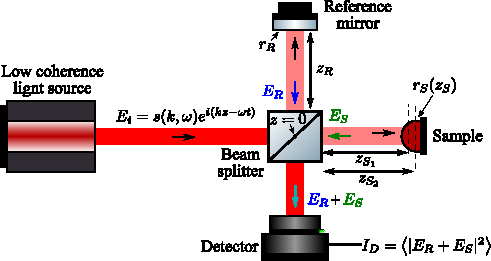
\includegraphics[width=.65\textwidth]{Figures/TheoreticalBasis/OCT_Model.pdf}
    \caption{Schematic of generic Michelson interferometer used in OCT.}
    \label{fig:OCT_Model}
\end{figure}

Interferometry measures the correlation between the electric fields of the light reflected by the sample and the reference mirror~\cite{Malacara2007_Optical}. Consider that the light source emits plane waves with electric field $E_i = s(k,\omega)e^{i(kz-\omega t)}$ at time $t$ and distance $z$ along the propagation axis, being $s(k,\omega)$ the complex amplitude, dependent on the angular frequency $\omega$ and wavenumber $k=2\pi / \lambda$ for wavelength $\lambda$. Assuming free space propagation and a 50/50 beam splitter, the reference beam propagates a distance $z_R$ from the beam splitter to the reference mirror with reflectivity $r_R$ and reflectance $R_R=|r_R|^2$, then reflected light propagates back to the beam splitter and its electric filed can be expressed as $E_R = \dfrac{E_i}{\sqrt{2}} r_R e^{i2kz_R}$.

On the other hand, light on the sample arm propagates a distance $z_S$ from the beam splitter to the sample. In biological tissues, the refractive index changes resulting in different reflectivities, therefore, the sample can be described as a discrete number $N$ of reflectors with reflectivities $r_{S_n}$ and reflectances $R_{S_n}=|r_{S_n}|^2$ located at distances $z_{S_n}$ as
\begin{equation}
    r_S(z_{S_n}) = \sum_{n=1}^N r_{S_n}\delta\left(z_S-z_{S_n}\right).
\end{equation}

\textbf{Coherent gating in OCT allows to reconstruct the function $\mathbf{\sqrt{R_{S_n}(z_{S_n})}}$ to produce images with optical contrast related to changes in the refractive index of the sample}~\cite{Izatt2015_Theory}.

Light backscaterred by the sample propagates back to the beam splitter with electric field $E_S=\dfrac{E_i}{\sqrt{2}}\sum\limits_{n=1}^Nr_{S_n}e^{i2kz_{S_n}}$. Reference and sample electric fields $E_R$ and $E_S$ interfere and a photodetector with responsivity $\rho$ captures the intensity producing a photocurrent $I_D(k, \omega)$ that can be described as~\cite{Izatt2015_Theory}
\begin{align}\label{eq:I_D(k,w)}
    I_D(k, \omega) &= \rho\left<\left|\frac{E_R}{\sqrt{2}} + \frac{E_S}{\sqrt{2}}\right|^2\right> \nonumber\\
    & = \rho\left<\left|\dfrac{E_i}{2} r_R e^{i2kz_R} + \dfrac{E_i}{2}\sum\limits_{n=1}^Nr_{S_n}e^{i2kz_{S_n}}\right|^2\right> \\
    & = \frac{\rho}{4}\left<\left|s(k,\omega) r_R e^{i2kz_R-\omega t} + s(k,\omega)\sum\limits_{n=1}^Nr_{S_n}e^{i2kz_{S_n}-\omega t}\right|^2\right>, \nonumber
\end{align}
assuming $z=0$ at the splitting surface of the beam splitter without loss of generalization, where $\left<\cdot\right>$ is the temporal averaging performed by the photodetector during the integration time of a single measurement, which is long enough to expect that $I_D$ is independent of the temporal component $\omega t$ given the fast temporal oscillation of light imposed by $\omega$. This is consequent with expansion of Eq.~\eqref{eq:I_D(k,w)} using $|E|^2 = E^*E$ that yields the spectral interferogram~\cite{Izatt2015_Theory}
\begin{align}\label{eq:I_D(k)}
I_D(k) &= \frac{\rho}{4}\left[S(k)\left(R_R + \sum_{n=1}^N R_{S_n}\right)\right] ... \nonumber\\
&+ \frac{\rho}{2} \left[S(k)\sum_{n=1}^N\sqrt{R_RR_{S_n}}\cos\left(2k\left[z_R-z_{S_n}\right]\right)\right] ... \\
&+ \frac{\rho}{4}\left[S(k)\sum_{n\neq m}^N\sqrt{R_{S_n}R_{S_m}}\cos\left(2k\left[z_{S_n}-z_{S_m}\right]\right)\right], \nonumber
\end{align}
where $S(k) = |s(k,\omega)^2|$ is the light source spectrum and $z_R-z_{S_n}$ is the OPL difference.

There are three components in $I_D(k)$ as noted in Eq.~\eqref{eq:I_D(k)}. First one is a \textit{background} component that is independent of propagating distances and it is the largest component given that typically reference mirror reflectivity denominates the sample reflectivity. In general, this is a undesired component that is canceled out using dual balanced detection~\cite{Podoleanu2000_Unbalanced}.

Second is a \textit{cross-correlation} component that depends on the spectrum of the light source $S(k)$, the wavenumber $k$ and the OPL difference $z_R-z_{S_n}$. This is the desired component in OCT imaging since it gives access to the sample reflectivity through the term $\sqrt{R_RR_{S_n}}$.

Last term is an \textit{auto-correlation} component that represents the interference between the different sample reflectors, independent of the reference light. This is commonly an artifact component that can be neglected increasing the magnitude of the other two components by increasing the reference mirror reflectivity.

Note that $I_D(k)$ in Eq.~\eqref{eq:I_D(k)} is the interference resulting from a particular wavenumber $k$, but the ultimate aim in OCT is to ``isolate'' the $\sqrt{R_RR_{S_n}}$ term along depth, i.e. versus OPL differences. There are two approaches to retrieve the depth-dependent photoccurent $i_D(z)$, yielding two major OCT configurations: time domain OCT (TDOCT)~\cite{Huang1991_Optical} and Fourier domain OCT (FDOCT)~\cite{Fercher1995_Measurement}.

\subsection{Time domain OCT}

Most straightforward way to obtain the depth-dependent signal is to use a mono-pixel detector to capture the interference while the reference delay $z_R$ is scanned by moving the reference mirror along the axial direction as shown in Figure~\ref{fig:TDOCT_Scheme}. The detector captures the intensity for all $k$ at the same time, thus $i_D(z_R)$ is the integration over all $k$ of $I_D(k)$~\cite{Izatt2015_Theory},
\begin{align}
    i_D(z_R) &= \frac{\rho}{4}S_0\left(R_R+\sum_{n=1}^N R_{S_n}\right)... \nonumber \\
    &+ \frac{\rho}{2}S_0 \sum_{n=1}^N \sqrt{R_RR_{S_n}} e^{-\left(z_R-z_{S_n}\right)^2 \Delta k^2}\cos\left[2k_0\left(z_R-z_{S_n}\right)\right],
\end{align}
where $S_0 = \int\limits_{0}^\infty S(k)dk$ is the spectral total power emitted by the light source, and a normalized Gaussian spectrum $S(k) =\dfrac{1}{\Delta k\sqrt{\pi}}e^{-\big[\frac{(k-k_0)}{\Delta k}\big]^2}$ is assumed, being $k_0$ the central wavenumber and $\Delta k$ the full-width at $1/e$ of the maximum.

\begin{figure}[htb!]
    \centering
    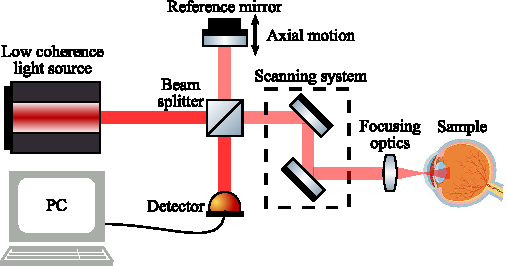
\includegraphics[width=.7\textwidth]{Figures/TheoreticalBasis/TDOCT_Scheme.pdf}
    \caption[Schematic of a generic TDOCT setup based on a Michelson interferometer.]{Schematic of a generic TDOCT setup based on a Michelson interferometer, where axial scan is performed by displacing the reference mirror in the axial axis while recording the interference with a mono-pixel detector.}
    \label{fig:TDOCT_Scheme}
\end{figure}

Time domain A-line $i_D(z_R)$ consists of a background component (DC), proportional to $S_0$, and an interference component that is a summation of Gaussian functions with finite width, having peak-values of $\sqrt{R_RR_{S_n}}$ located at OPL differences $z_R-z_{S_n}$ and modulated by cosines of period $\pi/k_0$, equivalent to $\lambda_0/2$. $\gamma(z_R)=e^{-(z_R-z_{S_n})\Delta k^2}$ is known as the \textit{coherence function} and it causes a ``broaning'' of the interference signal of each reflector and its width is related to the coherence length of the light source that determines the axial resolution, thus $\gamma(z_R)$ is considered as the axial point spread function (PSF)~\cite{Izatt2015_Theory}. Figure~\ref{fig:Alines} illustrates a TDOCT A-line in Fig.\ref{fig:Alines}(b) for a sample characterized by three reflectors as shown in Fig.\ref{fig:Alines}(a).

\begin{figure}[htb!]
    \centering
    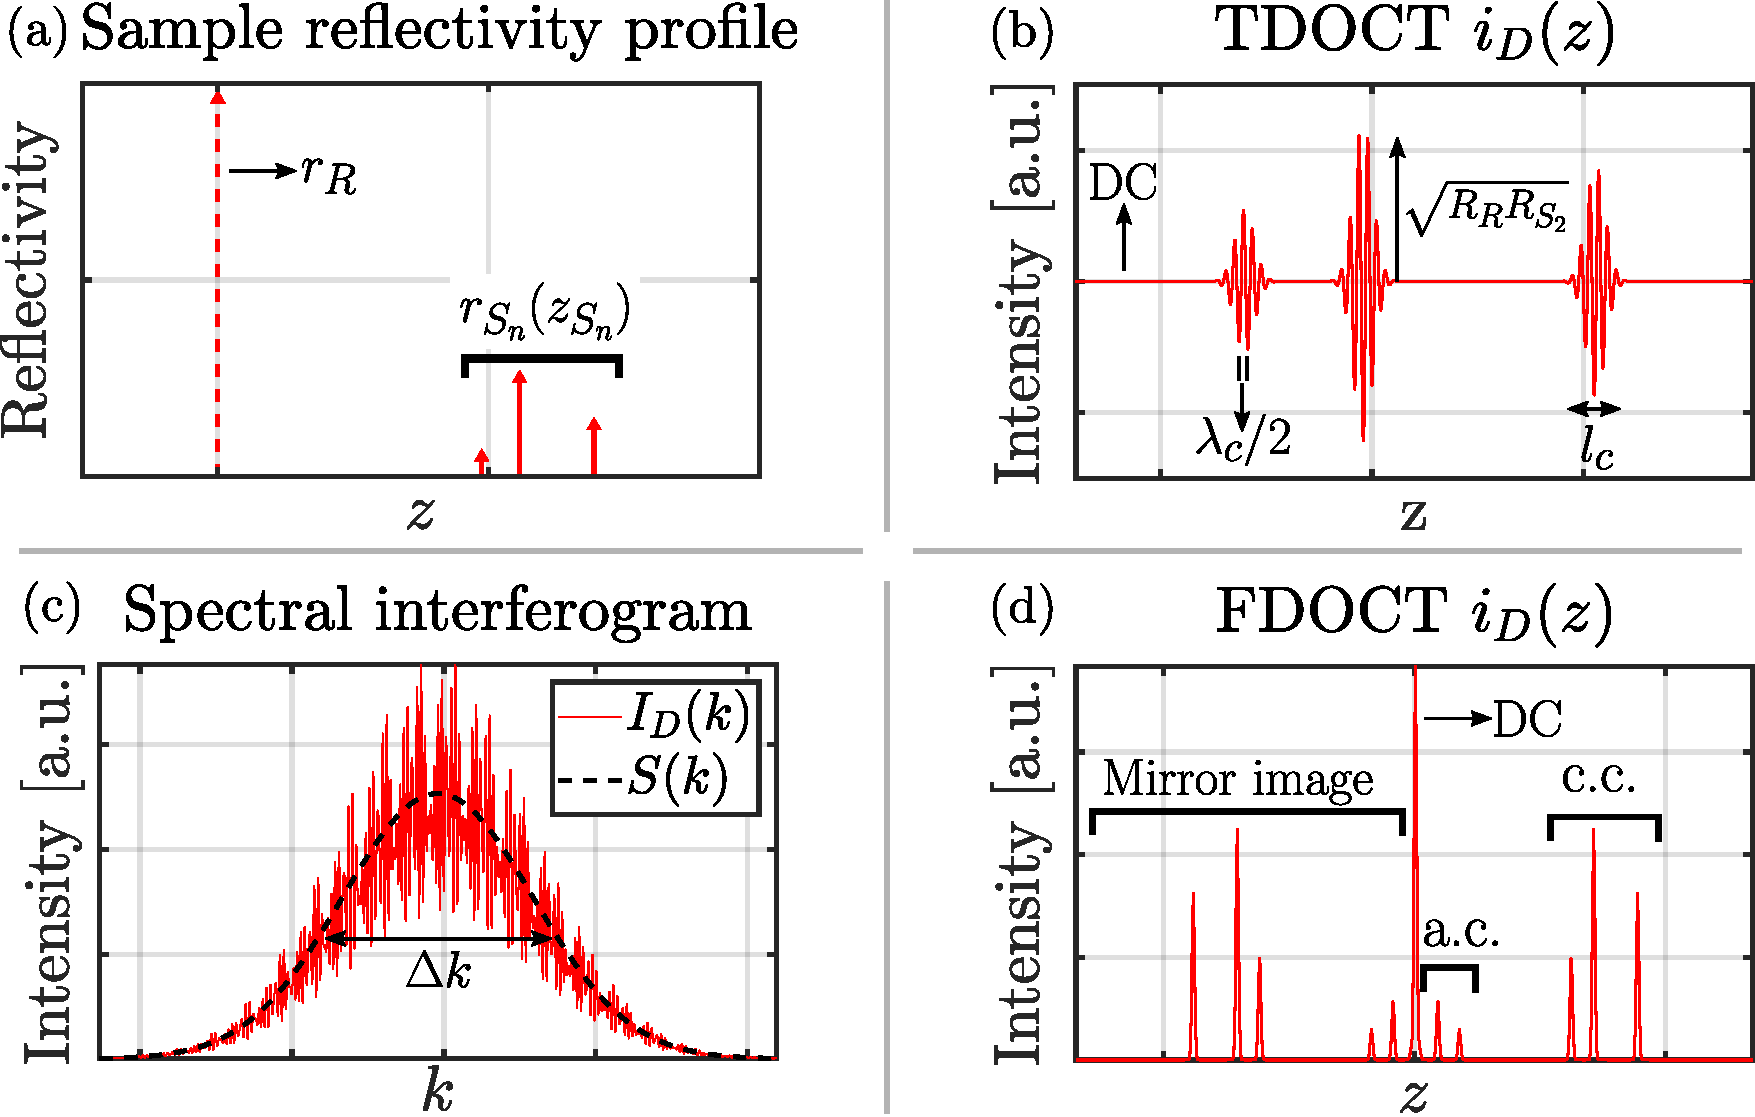
\includegraphics[width=.7\textwidth]{Figures/TheoreticalBasis/Alines.pdf}
    \caption[Illustration of A-lines obtained in OCT.]{Illustration of A-lines obtained in OCT. (a) Axial reflectivity profile for a sample characterized by three reflectors: (b) TDOCT A-line, (c) spectral interferogram and (d) FDOCT A-line obtained as the Fourier transform of (c), indicating the background (DC), cross-correlation (c.c.) and auto-correlation (a.c.) components.}
    \label{fig:Alines}
\end{figure}

Early OCT imaging systems including the first experimental demonstration of OCT in 1991~\cite{Huang1991_Optical} employed a time domain detection. Designation of time domain arises from the fact that the reflectivity axial profile of the sample is acquired while displacing the reference mirror in time. This demands mechanical systems to displace the reference mirror, which limits imaging speed to A-line rates $<\sim$2~kHz~\cite{Izatt2015_Theory}, due to technical restrictions to develop precise fast motion systems with micrometric resolution and millimetric travel range. Furthermore, given that axial scan is acquired while the detector captures the signal at different times, stable systems are required to avoid artifacts during imaging due to changes of the imaging system, for instance, changes of the light source emission. For this reason, achievable sensitivity is limited and this, in addition to low imaging speed, establishes the major drawbacks of TDOCT~\cite{Leitgeb2003_Performance}.

\subsection{Fourier domain OCT}

Although TDOCT systems served well in early medical OCT development, their relatively slow scan rate and limited sensitivity restricted the potential of OCT and restricted its expansion to many medical applications. An improvement in sensitivity and imaging speed in OCT was possible with the introduction of FDOCT systems where the reference mirror remains fixed~\cite{Choma2003_Sensitivity, Leitgeb2003_Performance, deBoer2003_Improved}. Axial spatial domain and optical frequency domain are conjugates with the wavenumber and the OPL difference being Fourier transform duals. This concept led to development of Fourier domain acquisition where photocurrent $I_D(k)$ in Eq.~\eqref{eq:I_D(k)} is captured directly in the $k$ space and a subsequent Fourier transform $\text{FT}_k\left\{\cdot\right\}$ of the signal  along variable $k$ yields the depth-dependent photocurrent $i_D(z)$, with not need to displace the reference mirror~\cite{Fercher1995_Measurement}.

Using the Fourier transform property $\text{FT}_k\left\{\cos(kz_0)\right\} = \frac{1}{2}\left[\delta\left(z+z_0\right) + \delta\left(z-z_0\right)\right]$, the convolution theorem $\text{FT}_k\left\{g\left(k\right)f\left(k\right)\right\} = \text{FT}_k\left\{g\left(k\right)\right\} \ast \text{FT}_k\left\{f\left(k\right)\right\}$, and the shifting property of delta functions $f(z)*\delta\left(z-z_0\right) = f(z_0)$, it is possible to obtain the FDOCT A-line $i_D(z) = \text{FT}_k\left\{I_D(k)\right\}$ from Eq.~\ref{eq:I_D(k)} as~\cite{Izatt2015_Theory}
\begin{align}\label{eq:i_D(z)}
    i_D(z) &= \frac{\rho}{8}\gamma\left(z\right)\left[R_R + \sum_{n=1}^NR_{S_n}\right] ... \nonumber\\
    &+ \frac{\rho}{4}\sum_{n=1}^N \sqrt{R_RR_{S_n}} \left[\gamma\left(2\left[z_R-z_{S_n}\right]\right) + \gamma\left(-2\left[z_R-z_{S_n}\right]\right)\right]...\\
    &+ \frac{\rho}{8}\sum_{n\neq m=1}^N \sqrt{R_{S_n}R_{S_m}} \left[\gamma\left(2\left[z_{S_n}-z_{S_m}\right]\right) + \gamma\left(-2\left[z_{S_n}-z_{S_m}\right]\right)\right], \nonumber
\end{align}
where again $\gamma\left(z\right)=\text{FT}_k\left\{S(k)\right\}$ is the coherence function of the source, that assuming a Gaussian emission spectrum is given by
\begin{align} \label{eq:SGamma}
    S(k) =\frac{1}{\Delta k\sqrt{\pi}}e^{-\big[\frac{(k-k_0)}{\Delta k}\big]^2} \xleftrightarrow{\hspace{8 pt}\text{FT}\hspace{8 pt}} \gamma(z) = e^{^{-z^2\Delta k^2}}.
\end{align}

Eq.~\eqref{eq:i_D(z)} contains three components as Eq.~\eqref{eq:I_D(k)}; background, cross-correlation and auto-correlation components. Figure~\ref{fig:Alines} shows an example of a Fourier domain A-line in Fig.~\ref{fig:Alines}(d) for a sample with three reflectors as shown in Fig.~\ref{fig:Alines}(a) and its corresponding interferogram in $k$ space in Fig.~\ref{fig:Alines}(c).

Cross-correlation component provides access to the signal of interest in OCT, $\sqrt{R_RR_{S_n}}$, by each reflector appearing at positions $\pm2(z_R-z_{S_n})$ and being ``broadened'' by the coherence function similarly to the case of the TDOCT A-line. The apparent position of the reflectors $\pm2(z_R-z_{S_n})$ have a factor of 2 since the interferometer measures the round-trip distance.

There is a ``mirror image'' produced by the fact that $I_D(k)$ is real, hence its Fourier transform is Hermitian symmetric, that is, the positive values are the complex conjugate of the negative values, and this is represented in the double sign of $\pm2(z_R-z_{S_n})$. This does not have an important influence if the sample is positioned entirely in one side of the zero OPL, such that it is possible to extract only one half of the Fourier spectrum to avoid the mirror image. 

Background component appears as a large component centered at the zero OPL. In general, it can be easily omitted from the signal since the reflectors of the sample are positioned beyond the zero OPL such that cross-correlation terms do not overlap with the background component. However, additional to the main lobe, side lobes may appear and cause significant artifacts overlapping with the cross-correlation terms, therefore, background is typically removed by recording the spectrum of the source blocking the light from the sample arm and then subtracting this background spectrum to every measurement.

Autocorrelation component appears near the zero OPL if the position of the reference mirror is such that $(z_{S_n}-z_{S_m}) << (z_R-z_{S_n})$, and this way it is possible to omit this artifact, but a more direct solution is to adjust the reference reflectivity to ensure that amplitude of cross-correlation terms are much higher than amplitude of auto-correlation terms.

Note that the OCT signal $i_D(z)$ is given as a function of depth for a specific transverse point with coordinates $(x,y)$ of the sample. In raster scan systems, the beam is scanned in the sample plane using galvanometer scan mirror that deflects the light beam changing its position in the sample, and in each location $(x,y)$ an A-line is acquired. Given that the interest so far is the axial scan, dependence on coordinates $(x,y)$ has been omitted for simplicity.
 
Sensitivity improvement in FDOCT with respect to TDOCT arises from the fact that interference for all depths are captured simultaneously, considering that the signal is acquired in $k$ space and it is known that each value in frequency domain contributes to all values in spatial domain~\cite{deBoer2003_Improved}. In FDOCT, there are two approaches to measure the spectral interferogram. Most intuitive way is to use a digital spectrometer as detector as shown in Figure~\ref{fig:SDOCT_Scheme}, which provides the intensity signal as a function of wavenumber $I_D(k)$ in a single measurement, and it is known as spectral domain OCT (SDOCT)~\cite{Fercher1995_Measurement}. Digital spectrometers are composed of a linear camera and an optical system that separates the spectral components of input light in such way that each pixel of the detector captures the intensity of a portion of the spectrum. Imaging speed in SDOCT is limited by acquisition rate of the linear camera and typical A-line rates are between 2 -- 50~kHz~\cite{Fujimoto2015_Introduction}.

\begin{figure}[htb!]
    \centering
    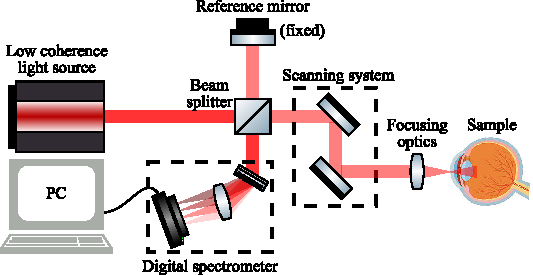
\includegraphics[width=.75\textwidth]{Figures/TheoreticalBasis/SDOCT_Scheme.pdf}
    \caption[Schematic of a generic SDOCT setup based on a Michelson interferometer.]{Schematic of a generic SDOCT setup based on a Michelson interferometer, where axial scan is obtained by computing the Fourier transform of the spectral interferogram acquired with a digital spectrometer.}
    \label{fig:SDOCT_Scheme}
\end{figure}

The second approach in FDOCT is to use a tunable light source with a narrow spectrum and to acquire the interference signal $I_D(k)$ with a single-element photodetector while the central emission wavenumber $k$ of the light source is swept among a broad spectrum, and it is known as wavelength-swept source OCT (SSOCT)~\cite{Chinn1997_Optical, Yun2003_Highspeed}. It is also referred as optical frequency domain imaging (OFDI)~\cite{Bouma2015_Optical} instead of low-coherence interferometry given that, in rigorous terms, instantaneous emission of the tunable light source is considered coherent. OFDI achieves the highest imaging speed in OCT, presenting A-line rates up to 200~kHz~\cite{Okabe2012_200}, or even more with specialized instrumentation~\cite{Oh2010_400}, and it is limited by the sweeping rate of the light source. Here OFDI and SSOCT are used indistinctly although in general OFDI is used to refer to the imaging technique and SSOCT is used to refer to the OCT systems itself. A more detailed description of SSOCT systems is provided below, because this is the one of interest for this work.

\subsection{Optical frequency domain imaging}

Operation of OFDI is grounded on the fact that OPL and wavenumber are conjugate variables. In low-coherence interferometry, interference is acquired illuminating the sample with light spanning several wavenumbers while OPL is scanned. In the alternative scenario, interference corresponding to all OPLs is acquired  at the same time, while illuminating the sample with light spanning a single wavenumber that is scanned, and this is the principle of operation of OFDI~\cite{Yun2003_Highspeed}. Then, a Fourier transform of the signal in spectral domain yields the depth-dependent signal.

Detection scheme in OFDI employs a single-element detector, allowing higher A-line rates than in SDOCT systems that are limited by the acquisition rate of the linear camera, which is composed of multiple pixels. Increasing imaging speed reduces motion artifacts when imaging \textit{in vivo} and allows larger scans in limited time. Tunable light sources are available in the 1--1.3~$\mu$m wavelength range, where cameras technology is not well established, hence SSOCT systems are used commonly in the 1--1.3~$\mu$m range that serves for multiple medical applications and SDOCT in the complementary 0.85--1~$\mu$m range used mainly in ophthalmology~\cite{Fujimoto2015_Introduction}.

The most relevant specifications of tunable light sources in SSOCT are repetition rate, instantaneous linewidth $\delta\lambda$, tunable range $\Delta\lambda$ and tuning curve $k_i(t)$~\cite{Yun2015_Wavelength}. Axial resolution is determined by central wavelength of emission $\lambda_c$ and tunable range $\Delta\lambda$ equally to Eq.~\ref{eq:axialRes}, $\delta_z = \frac{2\ln 2}{\pi}\frac{\lambda_c^2}{\Delta\lambda}$, thus it is independent of instantaneous linewidth. Instead, the depth range $\Delta z$ observed within a single A-line is determined by the instantaneous linewidth as
\begin{align}
\Delta z = \dfrac{\lambda_c^2}{4\delta\lambda}
\end{align}
and is independent of tunable range. Note that central wavelength mediate in both parameters. As a numerical example, a tunable light source with instantaneous linewidth $\delta\lambda=0.1$~nm and tunable range $\Delta\lambda=125$~nm centered at $\lambda_c=1.3~\mu$m provides $6~\mu$m axial resolution along $4.2$~mm depth range. The same light source but with central wavelength $\lambda_c=860$~nm provides $2.7~\mu$m axial resolution over $2.15$~mm.

Tunable curve $k_i(t)$ determines the instantaneous wavenumber as a function of time $t$. Ideally, this is a linear curve $k_i(t) = k_0 + k_st$ where $k_0$ is the initial wavenumber and $k_s$ is the wavenumber step between consecutive instantaneous wavenumbers~\cite{Dorrer2000_Spectral}. In practice, $k_i(t)$ is a non-linear function of time and thus linearization is required, typically performed on post-processing prior to computing the Fourier transform of the spectral interferogram, otherwise, artifacts appear degrading axial resolution~\cite{Dorrer2000_Spectral}.

Development of SSOCT systems have inherited technology from optical communications in the near infrared spectrum that employs similar optical components such as tunable laser sources, optical fiber and detectors~\cite{Yariv2007_Photonics}. In that sense, there are multiple types of tunable light sources relying on different principles of operations, but currently the development of fast, stable, linear, low-cost tunable light sources is a very active area of research~\cite{YasinAlibhai2018_Swept}.

Lasers are optical oscillators comprising a gain medium that is pumped optically or electrically to amplify light by stimulated emission, and an optical cavity that gives coherent optical feedback for laser oscillations~\cite{Saleh1991_Fundamentals}. Semiconductor optical amplifier (SOA) is a gain medium widely used for tunable lasers because they offer a high gain in a broad bandwidth, a rapidly response time, in the picosecond scale, and a wide range of gain center wavelengths depending on the semiconductor materials~\cite{Yun2015_Wavelength}. One way to construct tunable lasers is to incorporate in the basic laser instrumentation an internal or external scanning filter to select the central wavelength of the instantaneous emission. One of the first approaches developed for OCT applications is tunable lasers based on scanning filter using a polygonal mirror and to date this is widespread in research and medical systems~\cite{Yun2003_Highspeed}. Polygon-based tunable lasers offer high sweep rate in a wide tuning range with narrow linewidth, ideal features for OCT imaging.

In polygon-based lasers, the optical cavity includes a diffraction grating, a telescope and a rotating polygonal mirror with tens of facets~\cite{Yun2003_Highspeed}. Light emitted by a SOA within a broad spectrum is reflected by the diffraction grating in such way that there is an angular separation of spectral components. Light is relayed to the polygonal mirror through the telescope, and only the spectral component incident perpendicular to the mirror surface is reflected back to the grating and then to the SOA, providing a coherent light feedback. Rotation of the polygonal mirror changes surface angle and therefore the instantaneous spectral component that has perpendicular incidence also changes~\cite{Yun2003_Highspeed}. Drawbacks of this scanning filter approach is that polygonal mirror is a relatively bulky and moving part.

Figure~\ref{fig:SSOCT_Scheme} illustrates an optic fiber-based SSOCT system using a polygon-based tunable laser. Light from the tunable laser is delivered to an optic fiber beam splitter that divides the light into the sample and reference arms. Then, reflected light from both produce interference that is detected by a photodetector and digitized. In this scheme, balanced detection is illustrated using two detectors to subtract the background signal and thus suppressing excess noise\cite{Podoleanu2000_Unbalanced}. Moreover, SSOCT systems require a trigger signal to synchronize detector acquisition with rotation of the polygonal mirror~\cite{Vakoc2005_Phaseresolved}. In the system of Fig.~\ref{fig:SSOCT_Scheme}, the trigger signal is generated by a narrowband fiber Bragg grating (FBG) that reflects light of a specific wavelength, thus when the laser source emits this wavelength, the FBG reflects light generating a pulse that indicates the beginning of interferogram acquisition, performed using N analog-to-digital conversions (ADC) following a sample clock~\cite{Vakoc2005_Phaseresolved}.

\begin{figure}[htb!]
    \centering
    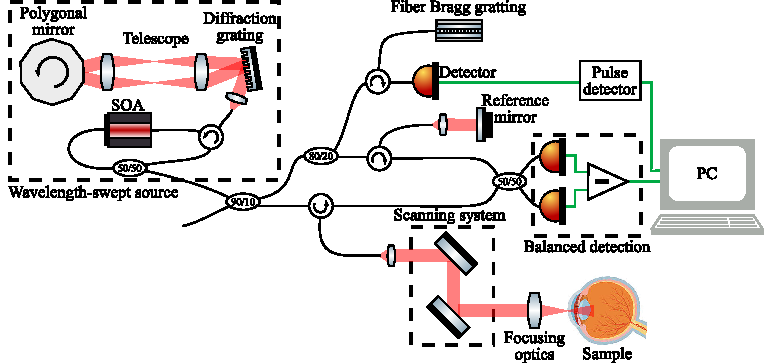
\includegraphics[width=\textwidth]{Figures/TheoreticalBasis/SSOCT_Scheme.pdf}
    \caption[Schematic of a fiber-based SSOCT setup.]{Schematic of a fiber-based SSOCT setup where the wavelength-swept source changes its instantaneous central wavelength in time due to the rotation of the polygonal mirror. A trigger signal to start the acquisition of the spectral interferogram is produced by the fiber Bragg grating that is designed to reflect a single wavelength, indicating the start of a sweep cycle of the light source.}
    \label{fig:SSOCT_Scheme}
\end{figure}

Compact tunable lasers have been possible with vertical cavity surface emitting lasers (VCSEL) in conjunction with a micro-electro-mechanical mirror system (MEMS) used to vary the cavity length of the VCSEL, thereby tuning the output wavelength~\cite{Vail1995_Tunable}. MEMS-VCSEL sources, however, have a limited tuning range and broad instantaneous linewidth although they are in current development to provide a powerful alternative to polygonal-based sources~\cite{Jayaraman2011_OCT}. In addition, current research focuses in developing akinetic tunable lasers to provide more robust and reliable light sources with the same or even better features of polygon-based sources~\cite{Lee2018_Akinetic}.

\subsection{Phase stability in OCT configurations}\label{sec:OCTConfigPhaseStab}

Being an interferometric technique, OCT provides information of the \textit{complex amplitude} of the light backscattered by the sample, and this includes phase and amplitude information. This is an important feature of OCT because the complex amplitude provides more information than the amplitude (or intensity) alone, enabling operation of phase-resolved functional techniques and phase-dependent post-processing~\cite{Park2020_Angiographic, Vakoc2005_Phaseresolved, White2003_vivo}.

In OCT, there are several undesired contributions to the phase that are considered as \textit{phase noise}, arising from the system or from the sample~\cite{Vakoc2005_Phaseresolved, Shemonski2014_Stability}, making development of phase-resolved OCT technology challenging. The ability of a system to provide repeatable phase measurements is known as \textit{phase stability} and it exists when there is a constant phase relation between measurements, that is, when the phase difference between entirely correlated measurements is zero~\cite{Shemonski2014_Stability}. In phase sensitive techniques like flowmetry, phase difference between consecutive measurements is directly related to the flow velocity, and phase stability is crucial because phase noise causing phase fluctuations adds spurious contribution to the calculation of the phase difference, inducing errors in the velocity estimation~\cite{White2003_vivo}.

Phase stability is greatly influenced by the configuration used for axial and transverse scan, and it is possible to obtain 1D (along one axis), 2D (along two axis), or 3D (volumetric) phase stability. In SDOCT, the parallel acquisition of the entire spectral interferogram within a single measurement ensures phase stability during acquisition of every A-line, thus axial axis is phase-stable. In addition, the high repeatability of spectrometers ensure phase stability along successive A-lines measured at different times, while scanning the beam in the sample, hence in principle SDOCT provides volumetric phase stability. However, there are additional sources of phase noise in OCT: one induced by sample motion that is detailed in Section~\ref{sec:phaseStab}, and second is induced in the galvanometer scanning system, due to separation of the pivot position of each galvanometer mirror and the back focal plane of the scan lens that adds a phase offset depending on the instantaneous angle of the mirror~\cite{Shemonski2014_Stability}. Although there is a physical limitation in positioning the pivot point of both galvanometers mirrors at the back focal length of the scan lens, precise alignment of one mirror would ensure phase stability along its corresponding lateral scan axis, resulting in 2D phase stability for SDOCT~\cite{Vakoc2009_Statistical}.

In SSOCT systems, achieving phase stability has been more challenging than in SDOCT because each component of the spectral interferogram is acquired sequentially in time and not in parallel like in a spectrometer. In principle, this is not a limitation if experimental conditions of the system during A-line acquisition do not change, but there is a particular issue in regard to the trigger signal that have a detrimental effect in phase stability. SSOCT systems require a trigger signal to synchronize A-line acquisition with the wavelength sweep of the light source~\cite{Vakoc2005_Phaseresolved}, for instance using a Fiber Bragg grating like in Fig.~\ref{fig:SSOCT_Scheme}. However, the fast sweeping cycle of the light source demand precise electronics to obtain a perfect synchronization, but in practice this is not the situation and there is a time delay or \textit{jitter} in the sample clock for acquisition with respect to the trigger signal. As a consequence, acquisition starts arbitrarily within the sweep cycle of the light source~\cite{Vakoc2005_Phaseresolved}.

A jitter in synchronization causes a shift $\delta k$ in the acquired spectral interferogram, thus the measured signal is $\tilde{I}_D(k) = I_D(k-\delta k)$. Depth-dependent signal obtained as $i_D(z)= \text{FT}_k\{\tilde{I}_D(k)\}$ results in~\cite{Hong2012_Highpenetration}
\begin{align} \label{eq:phaseJitter}
    \tilde{i}_D(z) &= \text{FT}_k\{I_D(k-\delta k)\} \nonumber \\
    &=  \text{FT}_k\{I_D(k)\} e^{-i2\pi z\delta k} \nonumber \\
    &=  i_D(z) e^{-i2\pi z\delta k},
\end{align}
being $i_D(z)=\text{FT}_k\{I_D(k)\}$ the unmodified depth-dependent A-line. Note that effect of spectral shift only impacts the phase of the A-line by the factor $e^{-i2\pi z\delta k}$ that represents a phase ramp with slope $-2\pi\delta k$, known as \textit{phase jitter} noise, but the amplitude $|\tilde{i}_D(z)|=|i_D(z)|$ remains unchanged, thereby traditional structural OCT image based on the intensity $|\tilde{i}_D(z)|^2=|i_D(z)|^2$ is not affected. The random behavior of jitter in synchronization causes that the spectral shift $\delta k$ varies randomly between spectral interferograms, and this dramatically impacts phase stability in raster scan systems because A-lines are captured sequentially in time while displacing the beam in the sample plane, inducing spatially-varying phase-jitter noise.

In addition to phase-jitter, random phase offsets can be induced in some SSOCT systems that are equipped with a frequency shifter used to eliminate the ambiguity between positive and negative optical path delays and hence doubling the axial imaging range~\cite{Yun2004_Removing}.

An approach to avoid phase-jitter is the use of $k$-clocks that produce a sample clock linear in $k$ using a Mach-Zehnder interferometer~\cite{Johnson2016_Multispeed}. In standard systems, signal acquisition is performed linearly in time with $N$ ADC following an internal electronic sample clock. With a $k$--clock, ADC are performed linearly in $k$ with certainty. Therefore, the use of a $k$--clock avoids phase-jitter because the uncertainty in trigger signal is solved, at the same time that acquired signal is linear in $k$ eliminating the need of signal linearization in post-processing. Although there are $k$-clocked SSOCT systems available~\cite{Kumar2017_Invivo}, they are not widespread because the need of additional hardware, thus phase-jitter is a very common issue affecting standard research and medical OCT systems~\cite{Bouma2015_Optical}. Additionally, even using a $k$-clock, SSOCT systems are sensitive to galvanometer and sample motion phase noise, affecting its phase stability~\cite{Shemonski2014_Stability-1}.

In the previous descriptions, it is possible to note that phase stability is very limited in raster scan systems, whether SDOCT or SSOCT, because transverse scan is performed in time. Parallel acquisition of A-lines for different transverse location can be achieved with extended-field systems where light is projected onto the sample in an extended area. In line-field SDOCT (LF-SDOCT), the sample is illuminated with a line-shaped beam, produced by a cylindrical lens, and the linear detector in the digital spectrometer is replaced by a two-dimensional detector: one dimension correspond to the $k$ space and the orthogonal dimension corresponds to the transverse fast scan axis~\cite{Nakamura2007_Highspeed, Ginner2017_Noniterative}. Hence, a single acquisition of the detector provides a B-scan view, and a single galvanometer is required to scan the beam along the slow scan axis providing three-dimensional images. Parallel acquisition along fast scan axis ensures phase stability \textit{in vivo} in this axis as long as acquisition rate is relatively fast compared to the velocity of the sample motion, nonetheless, slow scan axis typically remains phase-unstable~\cite{Ginner2017_Noniterative}.

TDOCT and SSOCT systems allow full field (FF) acquisition~\cite{Dubois2002_Highresolution, Hillmann2016_Aberrationfree} making three general modifications: an extended collimated beam is used to illuminate the sample; the single-element detector is replaced by a two-dimensional detector; and additional optical lenses are used to image the sample plane on the detector plane, and with these modifications a single axial scan provides an entire tomogram with volumetric phase stability, even \textit{in vivo} if acquisition rate is relatively fast compared to the velocity of the sample motion. Figure~\ref{fig:LF_FFOCT_Scheme} illustrates simple schematics of LF-SDOCT and FF-SSOCT systems.

\begin{figure}[htb!]
    \centering
    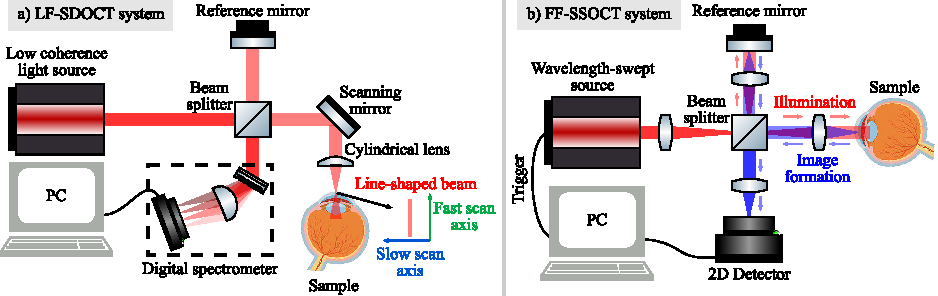
\includegraphics[width=\textwidth]{Figures/TheoreticalBasis/LF_FFOCT_Scheme.pdf}
    \caption[Schematic of generic LF-SDOCT and FF-OSCT setups.]{Schematic of generic (a) LF-SDOCT setup for acquisition of a B-scan in a single detector shot and (b) FF-SSOCT setup for acquisition of a tomogram in a single cycle of the wavelength-swept source. Red path illustrates the illumination beam and blue path the image formation on detector plane for a point.}
    \label{fig:LF_FFOCT_Scheme}
\end{figure}

Extended-field OCT systems are custom configurations used in particular scenarios, like in the CAC research area, because they offer sufficient phase stability~\cite{Kumar2013_Subaperture, Hillmann2016_Aberrationfree}, but they are not widespread given that they have a more complex optical design including 2D detectors that are not well developed in terms of speed and sensitivity in the near-infrared range, but more importantly, they are more prone to multiple scattering~\cite{Karamata2005_Multiple}. Scattered light in tissue can be divided into two components: single scattering and multiple scattering (MS). The former is the backscattered signal of interest in OCT and the latter is an undesired component arising from light that is scattered multiple times following random paths that reaches the detector, but it does not contribute direct information to the OCT signal due to its random properties~\cite{Karamata2005_Multiple-1}. Raster scan systems have an intrinsic rejection to MS because of confocal gating, that is, the focused beam scans a small region of the sample in a limited field of view (FoV), contrary to extended detection that is more prone to collect MS photons given that the FoV during each measurement is larger~\cite{Karamata2005_Multiple}.

There is not a general way to evaluate phase stability. Typically, assessment is performed by visually inspecting direct phase images, or more specifically histograms or images of phase differences between adjacent A-lines~\cite{Minneman2015_Akinetik}. Other possible quantitative approach is to image a coverslip or a reflective surface that is expected to have a constant phase, therefore the estimation of phase differences between consecutive A-lines yields an estimation of phase stability~\cite{Minneman2015_Akinetik}. One possible configuration to image the coverslip is to acquired A-lines while sweeping the beam with the galvanometer system, thus acquiring a B-scan, or simply by acquiring multiple A-lines at the same position with a static beam what is known as a C-scan. Typical, the standard deviation (STD) of phase differences is provided and used as a quantitative reference of phase stability. For instance, a phase stability of 0.32–5.2~mrad STD has been reported for SDOCT~\cite{White2003_vivo, Joo2005_Spectraldomain}, whereas 32~mrad STD has been reported for SSOCT systems using a polygon mirror-based laser~\cite{Manapuram2009_Phasesensitive} using phase stabilization methods, showing that this configuration is indeed more prone to phase instabilities than SDOCT, but a higher phase stability of 1.5~mrad STD using Akinetic swept laser has been obtained with SSOCT systems~\cite{Choi2013_Phasesensitive}.

\section{Modelling the acquisition of the complex OCT signal}\label{Model}

In previous section, OCT experiment was described and analyzed from an interference perspective to derive the acquisition of axial scan that provides the depth-dependent signal $i_D$ by means of optical interferometry. Hereafter, the OCT signal is represented by $S$ for consistency with general bibliography used to derive following models. The measured OCT signal $S$ corresponds to the complex field of light backscattered by the sample, however, the ultimate aim in OCT is not to know the backscattered light $S$ itself but to know the \textit{scattering potential} of the sample $\eta$ that produced the measured signal, because $\eta$ is directly related to the sample structure~\cite{Ralston2006_Inverse}. More specifically, in OCT the optical beam probe is used to measure $\eta$ indirectly; \textit{the acquired signal $S$ contains the sample scattering information modified by the effect of the optical system}. In the ideal situation, the effect of the optical system is not significant and the measured signal is directly related to $\eta$. This is the case of systems with aberration-free optical beams where imaging is diffraction-limited inside the depth of field and the theoretical lateral resolution is achievable, but in the presence of aberrations or outside the depth of field of the beam, the optical field is distorted and effective lateral resolution is reduced~\cite{Ralston2006_Inverse}.

Scattering theory can be used to derive a model of the imaging formation process that relates the measured signal with the sample structure, known as \textit{forward model}~\cite{Ralston2006_Inverse, Ralston2006_NonParaxial}. Inversion of the forward model results in the \textit{inverse scattering model} that allows to recover an approximate sample structure from the backscattering signal~\cite{Ralston2006_Interferometric}. Solutions to the inverse scattering model brought the development of computational techniques for aberration correction of OCT tomograms~\cite{Ralston2006_Interferometric, Yasuno2006_Noniterative, Adie2012_Computational}. In this section, the forward model is presented and subsequent section surveys solutions to the inverse scattering model to correct aberrations in post-processing, but first, a conceptual description of lateral-resolution--DoF trade-of is given.

\subsection{Confocal gating for lateral scan in OCT}

In raster scan systems, the transverse scan is performed using confocal gating resulting from the distribution of the focused beam as shown in Figure~\ref{fig:FocusingLens}. When light is focused on the sample plane, the illuminated cross-sectional area defines the lateral resolution and it can be given in terms of the input beam diameter~\cite{Yasuno2006_Noniterative}. Typically, at the back focal length of the optical system, the probe beam with central wavelength $\lambda_c$ is a Gaussian beam with a $1/e^2$--diameter $D$, and after the optical system, light is focused at the front focal length $f$ in a spot with a $1/e^2$--radius $w_0$, that defines the diffraction-limited lateral resolution $\delta x$~\cite{Fujimoto2015_Introduction}
\begin{align}
    \delta x = 2w_0 = \frac{4\lambda_c}{\pi} \frac{f}{D},
\end{align}
where $\dfrac{D}{2f} = \text{NA}$ is the numerical aperture of the optical system. The inverse relation of NA and $\delta x$ means that high NA systems produce small focused spots and therefore provide fine transverse resolution.

\begin{figure}[htb!]
    \centering
    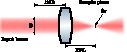
\includegraphics[width=.6\textwidth]{Figures/TheoreticalBasis/FocusingLens.pdf}
    \caption[Schematic of focusing optics in OCT.]{Schematic of focusing optics in OCT. Input collimated beam of diameter $D$ at the back focal length (BFL) is focused into focal point of diameter $\delta x$ at the front focal length (FFL).}
    \label{fig:FocusingLens}
\end{figure}

Due to convergence and divergence of the optical beam, the $1/e^2$--radius $w(z)$  of the focusing beam varies with depth $z$, and setting $z=0$ at the front focal plane, $w(z)$ ca be expressed as~\cite{Ralston2005_Deconvolution}
\begin{equation}\label{eq:beamWaist}
    w(z) = w_0 \sqrt{1 + \left(\frac{z\lambda_c}{\pi w_0^2n}\right)^2},
\end{equation}
where $n$ is the refractive index of the propagating medium.

Eq.~\ref{eq:beamWaist} shows that diffraction-limited resolution is only possible at the focal plane ($z=0$) and is degraded for other planes. However, for distances $z$ relatively close to the focal plane, change of spot size is relatively small. The confocal parameter $b$ is defined as the distance within which the spot size is smaller than $\sqrt{2}\delta x$ and thus resolution can be considered as nearly constant, and it is given by~\cite{Ralston2005_Deconvolution}
\begin{equation}
    b = 2z_R = \frac{\pi\delta x^2}{\lambda},
\end{equation}
where $z_R$ is known as the Rayleigh range. Confocal parameter defines the region where defocus is negligible and is also referred to as depth of field (DoF). It is proportional to the beam spot size squared and this establishes the lateral-resolution--DoF trade-off; high NA systems provides high resolution images in a limited DoF whereas low NA systems provides low resolution images in an extended DoF. In general, OCT systems employs low NA (between 0.01 and 0.15) to obtain tomograms with nearly focal resolution throughout the whole axial scan and this have limited transverse resolution in OCT to $\sim>10~\mu$m, although in certain applications high NA systems are used and known as optical coherence microscopy (OCM)~\cite{Fujimoto2015_Introduction}.

To illustrate confocal gating and its relation to numerical aperture, Figure~\ref{fig:ConfocalScan}(a) shows the focused beam produced by two optical systems in different NA regimes, for a wavelength $\lambda_c = 1~\mu$m. Low NA system (red) produces a large spot size but its size remains nearly constant along a large DoF. In contrast, the second system (blue) has a NA four times larger producing a spot size four times smaller but its size increases abruptly reducing the DoF by $4^2$ times. Fig.~\ref{fig:ConfocalScan}(b) shows the square relationship between confocal parameter and transverse resolution, indicating the corresponding values of the NA used in Fig.~\ref{fig:ConfocalScan}(a).

\begin{figure}[htb!]
    \centering
    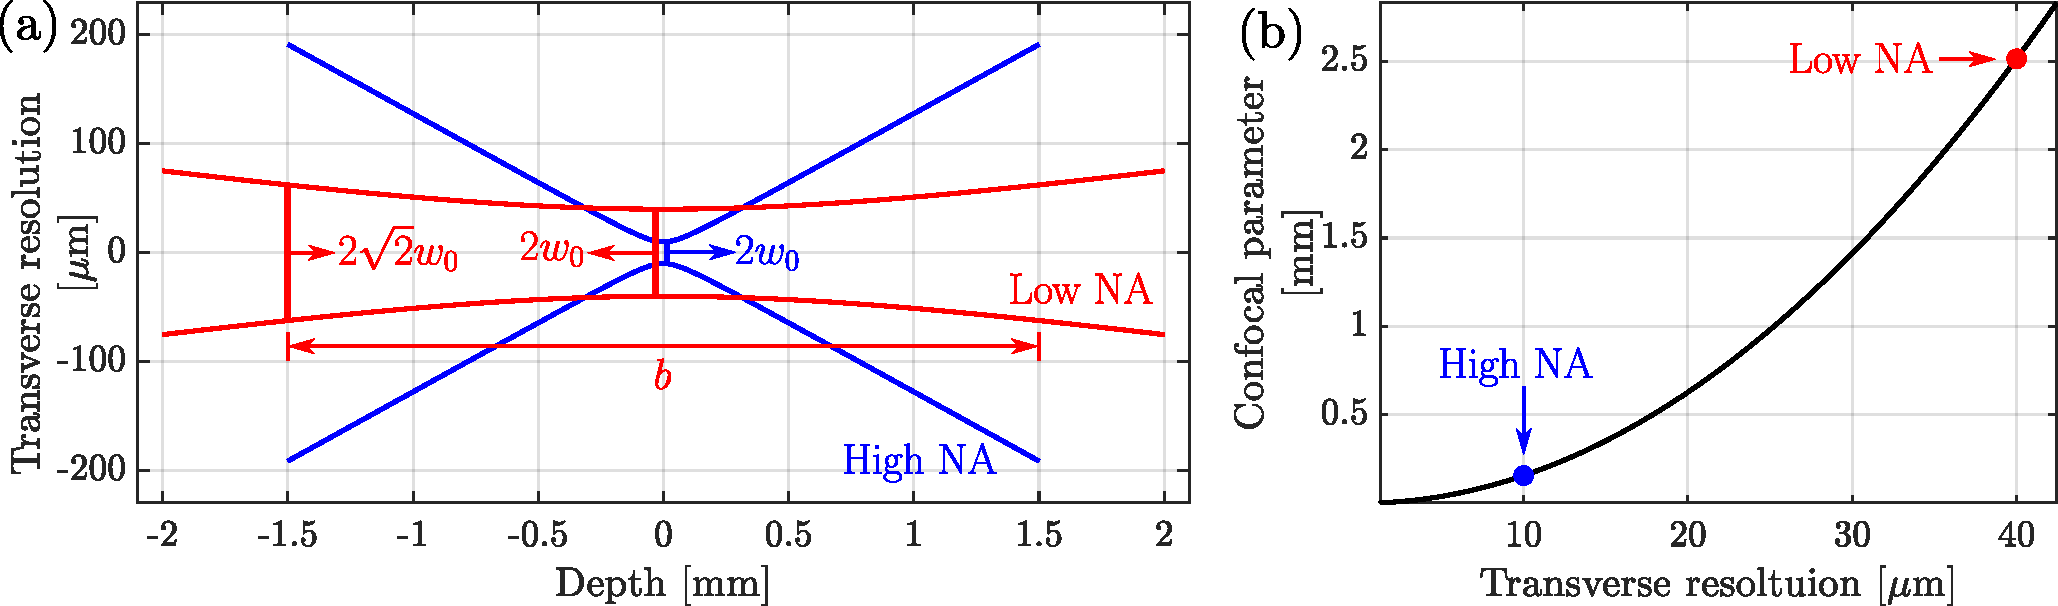
\includegraphics[width=\textwidth]{Figures/TheoreticalBasis/ConfocalScan.pdf}
    \caption[Illustration of confocal gating.]{Illustration of confocal gating for light with $\lambda_c = 1\mu$m. (a) Focused beam produced by two optical systems with relatively low and high NA. (b) Relation between confocal parameter and transverse resolution.}
    \label{fig:ConfocalScan}
\end{figure}

With this qualitative description of the resolution-DoF--trade-off, it is possible now to analyze how this impacts the acquired complex signal.

\subsection{Forward model}

This section presents the forward model (FM) that relates the measured OCT signal to the sample structure considering the effect of the optical system using a model for the image formation process. In the FM, the propagation of the Gaussian probe beam is taking into consideration to derive an expression for the interference signal that also considers the effect of confocal scan~\cite{Ralston2006_Inverse, Ralston2006_NonParaxial}. From Fourier optics theory, the acquired signal $S(x,y; k)$ for wavenumber $k$ at transverse coordinates $(x,y)$ can be modelled as $S(x,y; k)= h(x,y,z; k)\otimes\eta(x,y,z)$, that is the convolution (denoted by $\otimes$) of the system coherent point spread function (PSF) $h(x,y,z; k)$ with the scattering potential of the sample $\eta(x,y,z)$~\cite{Davis2007_Nonparaxial},
\begin{equation}\label{eq:conv}
    S(x,y; k) = \iiint h(x-x', y-y', z'; k) \eta(x',y',z') \text{d}x' \text{d}y' \text{d}z',
\end{equation}
where the integration over $z'$ indicates that light is captured simultaneously for all depths, as occurs in Fourier domain detection. Strictly speaking, $h(x,y,z; k)$ is the system's impulse response, but it is typically denoted simply as the PSF~\cite{Adie2015_Interferometric}. $h(x,y,z; k)$ can be expressed as the product of the incident and detection complex probe beams, $g_i(x,y,z;k)$ and $g_d(x,y,z;k)$ respectively, but given that OCT is based on a reflection (double-pass) geometry, the incident and collection beams are identical to $g(x,y,z;k)$, hence~\cite{Ralston2006_Inverse}
\begin{equation}\label{eq:PSF1}
    h(x,y,z; k) =k^2|A(k)|^2g^2(-x, -y, z; k),
\end{equation}
where $|A(k)|^2$ is the power spectral density and the inversion of lateral coordinates $(x,y)$ is due to the reflection geometry.

To derive a model for the probe beam $g(x,y,z;k)$, consider that the beam at the focal plane $z=z_0$ and transverse coordinate $\mathbf{r_0} = (x,y,z_0)$ is a normalized Gaussian probe beam
\begin{equation}\label{}
    g_0(\mathbf{r_0}; k) = \frac{1}{2\pi w_0^2(k)}e^{-\mathbf{r_0}^2/[2w_0^2(k)]},
\end{equation}
with waist radius $w_0(k) = \alpha / k$ for wavenumber $k$ and $\alpha = \pi/\text{NA}$. Using plane-wave decomposition with transverse frequency coordinate $\mathbf{q} = (q_x, q_y, 0)$, the beam at $\mathbf{r} = (x, y, z)$ in any plane $z$ is described as~\cite{Ralston2006_Inverse}
\begin{equation}\label{}
    g(\mathbf{r}; k) = \frac{1}{(2\pi)^2} \iint e^{i(z-z_0)\sqrt{k^2 - \mathbf{q}^2}} e^{-\mathbf{q}^2\alpha^2/2k^2} e^{i\mathbf{q}\cdot\mathbf{r}} \text{d}^2\mathbf{q}.
\end{equation}

Using Eqs.~\ref{eq:conv} and \ref{eq:PSF1}, it is possible to model the measured OCT interference signal taking into consideration the beam distribution, as explained in detail in Refs.~\cite{Ralston2006_Inverse, Marks2006_Inverse}, by means of the expression
\begin{equation}\label{eq:FM}
    S(\mathbf{r'}; k) = \frac{A(k)}{(2\pi)^2 k} \iiint f^2(\mathbf{r}-\mathbf{r'}; k) \eta(\mathbf{r}) \text{d}^2\mathbf{r} \text{d}z,
\end{equation}
where the term $f^2(\mathbf{r}; k)$ is given by
\begin{equation}\label{eq:f^2}
    f^2(\mathbf{r}; k) = \frac{1}{8\pi^2}\left(\frac{\alpha^2}{k^2}+\frac{iz}{k}\right)^{-1} \iint e^{-\mathbf{q}^2\alpha^2/4k^2} e^{iz\sqrt{4k^2-\mathbf{q}^2}} e^{-i\mathbf{q}\cdot \mathbf{r}} \text{d}^2\mathbf{q}.
\end{equation}

To understand Eq.~\ref{eq:FM}, note that $\mathbf{r'}=(x',y',z_0)$ is the instantaneous transverse position of the probe beam during a raster scan. The signal $S(\mathbf{r'},k)$ measured for the instantaneous wavenumber $k$ when the beam is located at the instantaneous position $\mathbf{r'}$, \textbf{is the contribution of all point scatterers in the sample weighted by the function $f^2(\mathbf{r}-\mathbf{r'}; k)$}, and scaled by a value proportional to the light source intensity for $k$, $A(k)$. Finally, a Fourier transform of $S(\mathbf{r'}; k)$ with respect to $k$ yields the depth-dependent signal $S(\mathbf{r'}, z)$. In regard to $f^2(\mathbf{r}-\mathbf{r'}; k)$, the factor $\frac{1}{8\pi^2}\left(\frac{\alpha^2}{k^2}+\frac{iz}{k}\right)^{-1}$ can be considered as a depth-dependent signal-loss factor that describes the signal reduction far from the focal plane, $e^{-\mathbf{q}^2\alpha^2/4k^2}$ is related to the Fourier spectrum of the Gaussian beam, the factor $e^{iz\sqrt{4k^2-\mathbf{q}^2}}$ encompasses both the interference and the PSF broadening effect, responsible of the signal blurring, and last factor $e^{-i\mathbf{q}\cdot \mathbf{r}}$ is the Fourier transform kernel as Eq.~\ref{eq:f^2} is actually a Fourier integral.

To illustrate the forward model, Figure~\ref{fig:FM1} shows an example of an OCT B-scan image simulated using Eq.~\ref{eq:FM}. For this purpose, a collection of $128$ point scatterers with random positions where defined within an axial and lateral field of view (FoV) of $820\times 450~\mu$m as depicted in Fig.~\ref{fig:FM1}(a). The light source have $\Delta\lambda=150$~nm and $\lambda_c=1.310~\mu$m providing an axial resolution of $\delta z=5~\mu$m. The numerical aperture is NA $= 0.25$, a relatively high value, resulting in lateral resolution $\delta x=5~\mu$m throughout a depth of field of $b=30~\mu$m, producing the Gaussian beam shown in Fig.~\ref{fig:FM1}(b), where the focal plane is clearly located at $z_0=0$. To generate the simulated OCT image shown in Fig.~\ref{fig:FM1}(c), the location of the Gaussian beam is changed iteratively, and in each location the contribution of all point scatterers weighted by $f^2(\mathbf{r}-\mathbf{r'}; k)$ is computed using Eq.~\ref{eq:FM}. At the $n$-th iteration, the location of the Gaussian beam is $\mathbf{r}'_m=(n\text{d}x - \frac{\Delta x}{2},0,z_0)$, where $\Delta x$ is the lateral FoV and $\text{d}x = 1.75~\mu$m is the sampling step which is smaller than Nyquist sampling, given by $\delta x / 2$, in order to fulfill Nyquist theorem for correct sampling.

\begin{figure}[htb!]
    \centering
    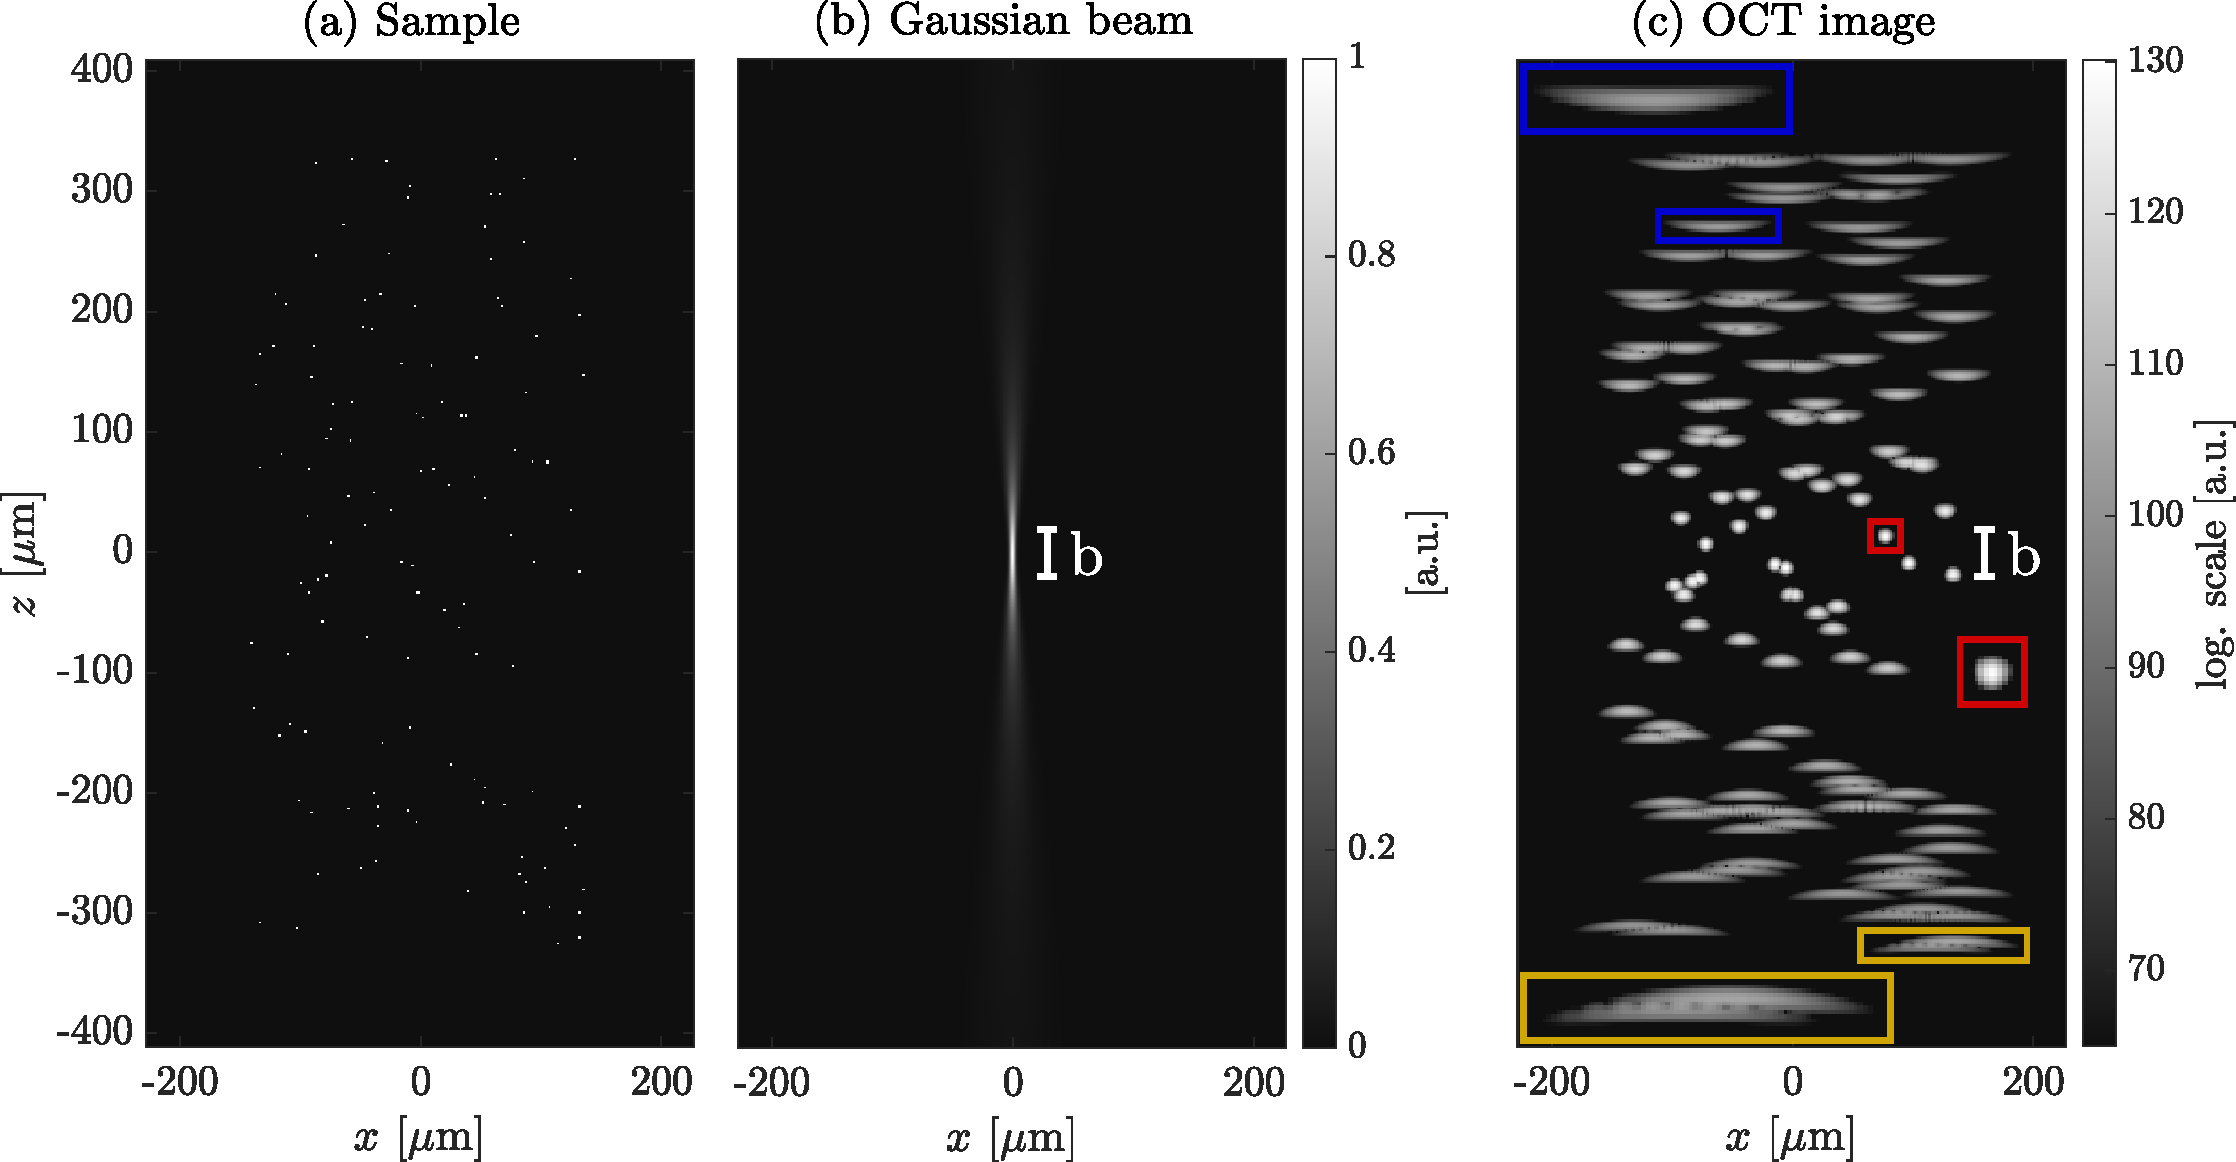
\includegraphics[width=\textwidth]{Figures/TheoreticalBasis/FM-HighNA.pdf}
    \caption[Simulation of an OCT image in high-NA regime.]{Simulation of an OCT image in high-NA regime. (a) Sample consisting of randomly located point scatterers, (b) Gaussian beam of the system with NA$=0.25$ and (c) OCT image simulated using the forward model, displayed in logarithmic scale.}
    \label{fig:FM1}
\end{figure}

The lateral blurring due to the convergence and divergence of the probe beam is evident in Fig.~\ref{fig:FM1}(c). Resolution within the confocal region marked as $b$ is diffraction-limited, so that point scatterers inside $b$ appear in focus, like the one inside the red rectangle, contrary to point scatterers away from the focal plane that appear blurred in the lateral axis as a consequence of beam size increase, such as the one in the blue rectangle. Note that superposition of signal from different point scatterers cause interference, like the two superimposed points in the yellow rectangle. When the number of point scatterers increases, random interference occurs and this phenomenon gives rise to speckle~\cite{Goodman2007_Speckle}.

It is important to remark that confocal effect is not restricted to the lateral axis. The factor $e^{iz\sqrt{4k^2-\mathbf{q}^2}}$ in Eq.~\eqref{eq:f^2} can be written as $e^{izq_z(k, \mathbf{q})}$, where $q_z=\sqrt{4k^2-\mathbf{q}^2}$ is the axial frequency coordinate of the object~\cite{Davis2007_Nonparaxial}. Because $q_z$ encompasses $k$ and $\mathbf{q}$, there is a mixing of the lateral and axial information that produces a coordinate warping, from the sample frequency coordinates $(q_x, q_y, q_z)$ to the signal frequency coordinates $(q_x, q_y, k)$~\cite{Ralston2006_Inverse}. As a consequence, there is an apparent object curvature away from the focal plane as observed in the blue inset of Fig.~\ref{fig:FM1}(c). The signal warping occurs because the object axial frequency component $q_z$ is not measure directly but through the light wavenumber $k$~\cite{Fercher2003_Optical}. In other words, the object frequency content is in the $(q_x, q_y, q_z)$ space, but the measured signal is the $(q_x, q_y, \frac{1}{2}\sqrt{q_x^2 + q_y^2 + q_z^2})$ space. This phenomenon is significant in high NA regime, and for low-NA regime an approximation can be made to simplify the FM as will be discussed in the next section.

For a comparison between high and low NA regimes, Figure~\ref{fig:FM2} illustrates the result of imaging the same sample of Fig.~\ref{fig:FM1}(a) changing the NA to $0.1$, resulting in a lateral resolution of $ 12.5~\mu$m throughout a depth of field of $190~\mu$m. The Gaussian beam produced with this NA have a more constant beam size along depth, as shown in Fig.~\ref{fig:FM2}(b) in contrast to the previous NA used for Fig.~\ref{fig:FM1}(b). As a result, resolution loss away from the focal plane is less abrupt, at the expense of presenting a larger diffraction-limited spot size.

\begin{figure}[htb!]
    \centering
    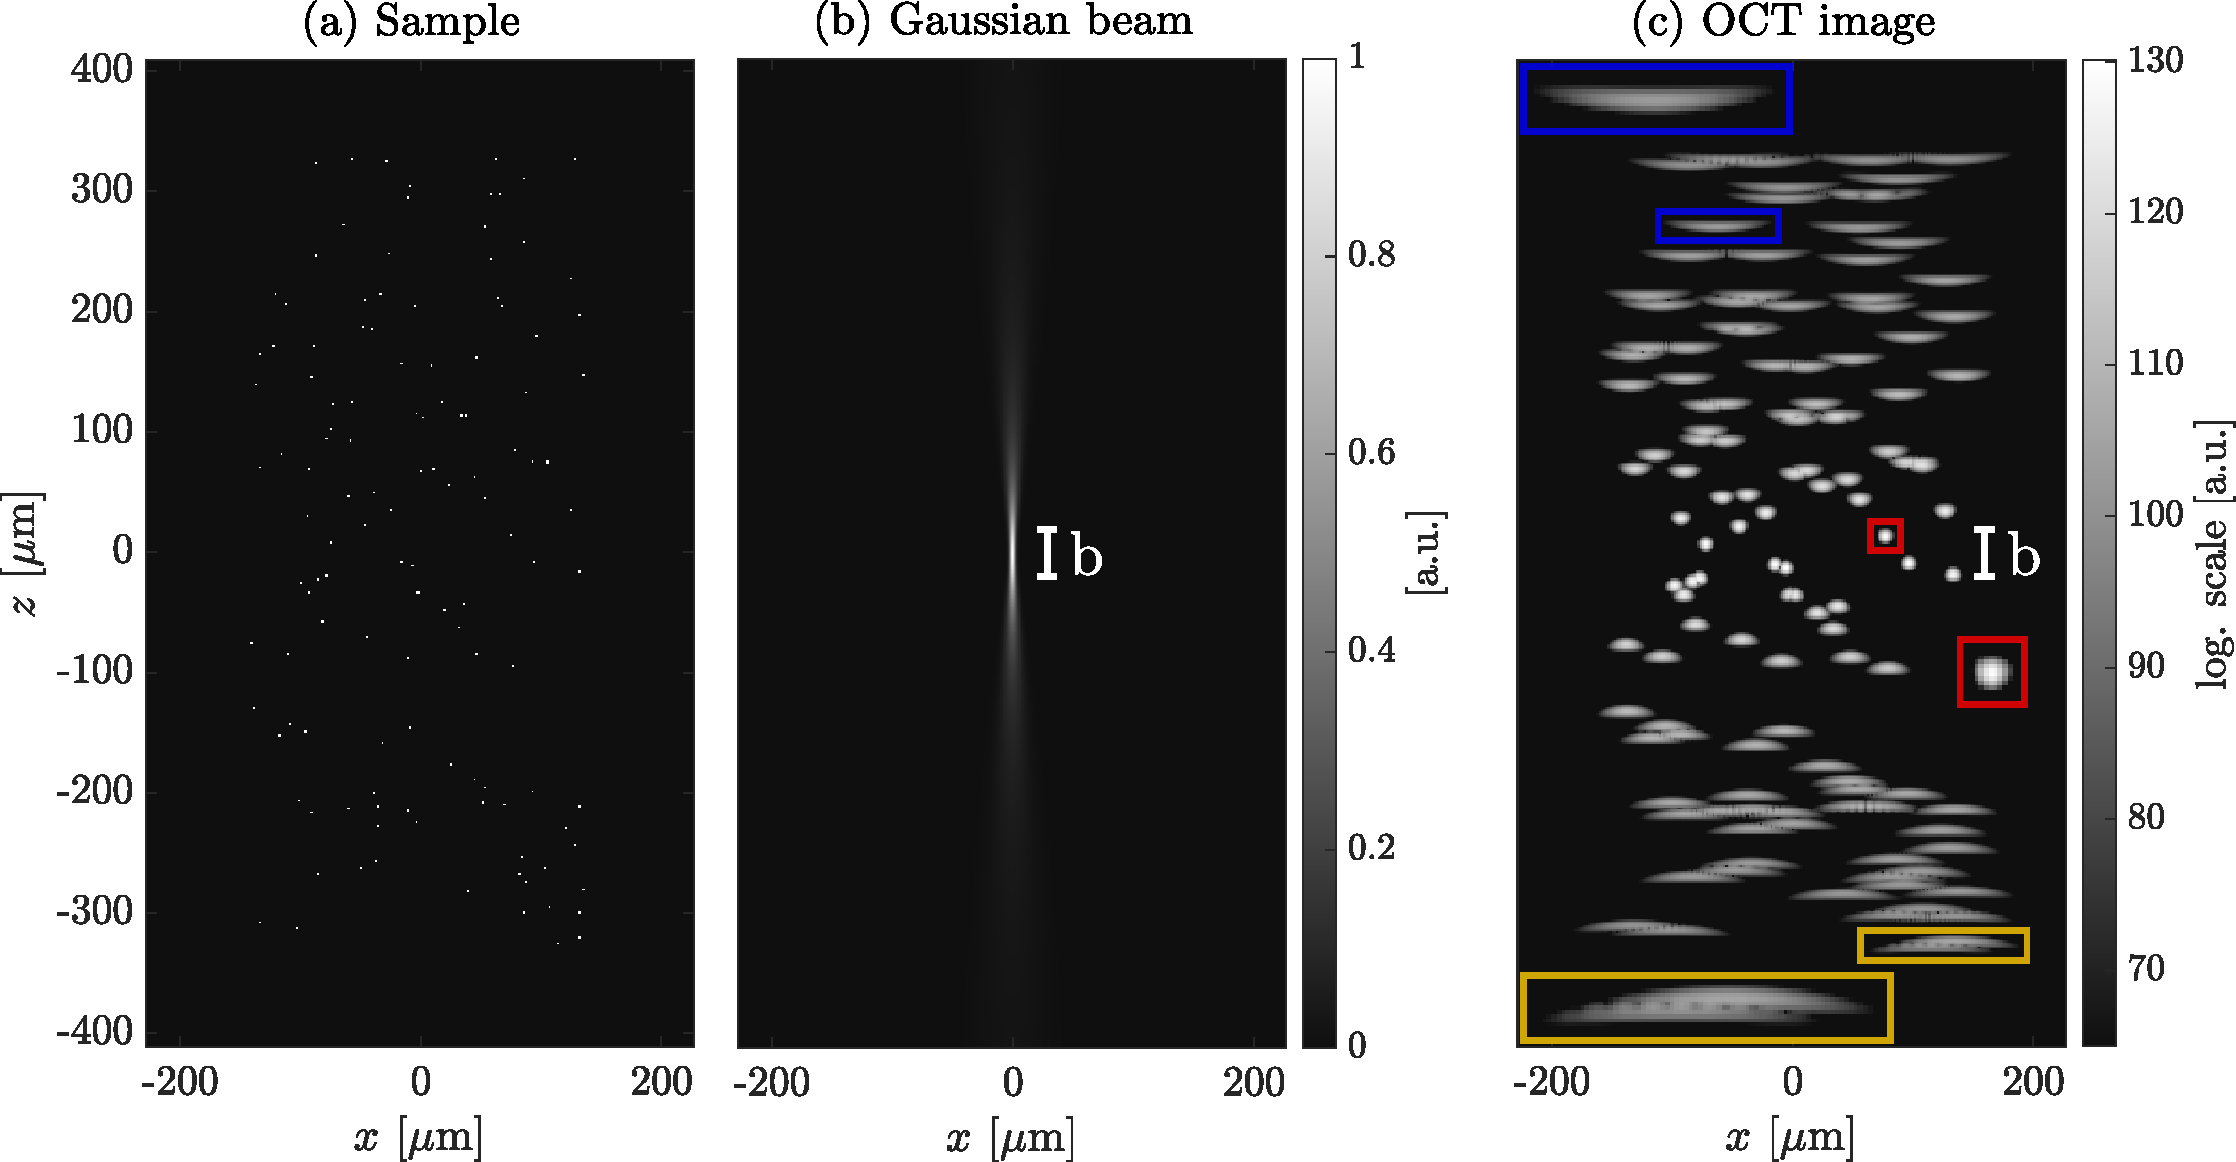
\includegraphics[width=\textwidth]{Figures/TheoreticalBasis/FM-LowNA.pdf}
    \caption[Simulation of an OCT image in low-NA regime.]{Simulation of an OCT image in low-NA regime. (a) Sample consisting of randomly located point scatterers, (b) Gaussian beam of the system with NA$=0.1$ and (c) OCT image simulated using the forward model, displayed in logarithmic scale.}
    \label{fig:FM2}
\end{figure}

% \iffalse Eq.~\ref{eq:conv} can be simplified in Fourier domain by invoking the convolution theorem and denoting the 2D Fourier transform over coordinates $(u, v)$ as $\text{FT}_{u,v}\{\cdot\}$,
% \begin{equation}\label{eq:convFT}
%     \hat{S}(q_x, q_y; k) = \int \hat{h}(q_x, q_y, z'; k) \hat{\eta}(q_x, q_y, z') dz'
% \end{equation}
% where $\hat{S} = \text{FT}_{x,y}\{S\}$, $\hat{h} = \text{FT}_{x,y}\{h\}$, $\hat{\eta} = \text{FT}_{x,y}\{\eta\}$, and $(q_x,q_y)$ are spatial frequency coordinates.

% The PSF can be expressed as the product of the incident and detection complex probe beams, and given that OCT is based on a reflection (double-pass) geometry, the incident and collection beams are identical to $\sqrt{\mu_r}k|A(k)|g(x,y,z;k)$, where $\mu_r$ is the beam splitting power ratio, $|A(k)|^2$ is the power spectral density, and $g(x,y,z; k)$ is the focused beam produced by an input collimated beam at the back focal length of the optical system, thereby
% \begin{equation}\label{eq:PSF1}
%     h(x,y,z; k) = \mu_rk^2|A(k)|^2g^2(-x, -y, z; k),
% \end{equation}
% where the inversion of lateral coordinates $(x,y)$ is due to the reflection geometry. 

% A plane wave decomposition of the focused probe beam yields~\ref{}
% \begin{equation}~\label{eq:planewavedecomp}
%     g(x,y,z ;k) = \frac{-i}{2\pi}\iint \frac{G(q_x, q_y, k)}{k_z}e^{i(q_xx+q_yy+k_zz)} dq_xdq_y,
% \end{equation}
% in terms of the generalized pupil function of the optical system $G(q_x, q_y, k)$, the object spatial frequencies $(q_x, q_y)$ and with $k_z(q_x, q_y) = \sqrt{k^2 - q_x^2 - q_y^2}$ that results from considering the optical wave vector $\mathbf{k}=(q_x, q_y, k_z)$.

% The 2D Fourier transform over coordinates $(q_x, q_y)$ of Eq.~\ref{eq:planewavedecomp}, $\hat{g} =  \text{FT}_{x,y}\{g\}$, results in
% \begin{equation}\label{eq:gFT}
%     \hat{g}(q_x, q_y, z; k) = -i2\pi\frac{G(q_x, q_y; k)}{k_z(q_x, q_y)}e^{izk_z(q_x, q_y)}
% \end{equation}

% Now, computing the 2D Fourier transform over coordinates $(q_x, q_y)$ of Eq.~\ref{eq:PSF1} and using the convolution theorem, note that the transverse transfer function $\hat{h} \propto \hat{g} \otimes\hat{g}$ and it can be expressed using Eq.~\ref{eq:gFT} as
% \begin{align}\label{eq:hFT}
%     \hat{h}(-q_x, -q_y, z; k) = -4\pi^2\mu_rk^2|A(k)|^2  &\iint \frac{G(q_x', q_y'; k)}{k_z(q_x', q_y')} \frac{G(q_x-q_x', q_y-q_y'; k)}{kz(q_x-q_x', q_y-q_y')}... \nonumber\\
%     &\times e^{-izk_z(q_x', q_y')}e^{-izk_z(q_x-q_x', q_y-q_y')}dq_x'dq_y'
% \end{align}

% To solve the integral in Eq.~\ref{eq:eq:hFT} it is possible to consider two complementary situations; near- and far-from-focus regimes. Recalling that $z=0$ at the focal plane, the far-from-focus regime is valid outside the DoF where effect of defocus is significant, where $z$ becomes large hence the phase term $|zk_z(q_x',q_y')|$ causes a rapid oscillation of the exponential term. This consideration allows to make use of the method of stationary phase~\ref{} which applies for integrals containing a rapidly oscillating complex exponential, such that the solution of the integral is found by evaluating the integral in the stationary point~\ref{}, that is, the point at which the argument of the complex exponential has zero gradient. The approximation of integral in Eq.\ref{eq:hFT} using the stationary point $(q_x', q_y') = (q_x/2, q_y/2)$ is
% \begin{equation}\label{eq:hFT_fff}
%     \hat{h}(-q_x, -q_y, z; k) \approx \frac{i4\pi}{-z}\mu_rk|A(k)|^2G^2\left(\frac{q_x}{2}, \frac{q_y}{2}; k\right)e^{-i2zk_z(\frac{q_x}{2}, \frac{q_y}{2})}.
% \end{equation}

% This expression shows explicit the amplitude and phase of the transverse transfer function of the system. The factor of $i=e^{i\frac{\pi}{2}}$ is equivalent to a phase of $\frac{\pi}{2}$ that is known as Gouy phase shift and it is characteristic of focused Gaussian beams~\ref{}. Decaying factor $1/z$ represents the signal decay with distance from focal plane that explains the loss of signal strength outside the DoF. In addition to the previous term, the other phase-dependent term is the phase factor that is responsible for the degradation of transverse resolution with increasing distance to the focal plane.

% For the near-focus regime, consideration to apply the method of stationary phase to solve the integral in Eq,~\ref{eq:hFT} is not longer valid. In this case, $z$ is small hence the phase term $|zk_z(q_x',q_y')|$ oscillates slowly and the term $G(q_x', q_y'; k)$ can be considered narrowly peaked compared to the slow oscillation of the exponential term, and this can be used to derive an approximation solution~\ref{}, however, the derivation is rather extensive as explained in detail in Ref.~\ref{} and superfluous in this context considering that inside the DoF defocus correction is unnecessary when compared to the far-from-focus regime.

% To finally derive the forward model for the far-from-focus regime, the transfer function of the system in Eq.~\ref{eq:hFT_fff} is replaced in Eq.~\ref{eq:convFT} to obtain
% \begin{equation}\label{eq:SFT}
%     \hat{S}_F(q_x, q_y; k) =  H_F(q_x, q_y; k)\int \frac{\tilde{\eta}(q_x, q_y, z')}{-z'}e^{-i2z'k_z(\frac{q_x}{2}, \frac{q_y}{2})} dz'.
% \end{equation}
% where $H_F(q_x, q_y; k) = i4\pi\mu_r k |A(k)|^2 G^2(-\frac{q_x}{2}, -\frac{q_y}{2}; k)$ is the depth-independent component of $\hat{h}$. Eq.~\ref{eq:SFT} is in the form of a Fourier transform with conjugate coordinates $z'$ and $2k_z(\frac{q_x}{2}, \frac{q_y}{2})$ and filtered by $H_F$. In fact, it has been proven that the forward model for the near-focus regime follow the same form that the forward model for far-from-focus, except that the Gouy phase shift and the decaying term $-1/z$ are not present and the depth-independent component of $\hat{h}$, denoted by $H_N(q_x, q_y; k)$, follows a slightly different functional form as can be seen in Ref.~\ref{}. Therefore, an unified approximate forward model for near- and far-from-focus regimes can be expressed in frequency domain as
% \begin{equation}\label{eq:FM}
%     \hat{S}(q_x, q_y; k) = H(q_x, q_y; k)\doublehat{\eta_a}(q_x, q_y, q_z)
% \end{equation}
% where $\doublehat{\eta_a}(q_x, q_y, q_z) = \text{FT}_{x,y,z}\{\rho(z)\eta(x,y,z)\}$ is the 3D Fourier transform of the attenuated scattering potential with spatial frequency coordinates $(q_x, q_y, q_z)$ where $q_z = -2\sqrt{k^2 - \left(\dfrac{q_x}{2}\right)^2 - \left(\dfrac{q_y}{2}\right)^2}$, and with the unified functions $H$ and $\rho$ given by
% \begin{equation}
% H(q_x, q_y; k) = 
% \begin{cases}
%     H_N(q_x, q_y; k)~~~\text{for}~~~|z| \ll z_R, \\
%     H_F(q_x, q_y; k)~~~\text{for}~~~|z| \gg z_R,
% \end{cases}
% \end{equation}
% \begin{equation}\label{eq:rhoz}
% \rho(z) = 
% \begin{cases}
%     ~1~~~~~\text{for}~~~|z| \ll z_R, \\
%     -\dfrac{1}{z}~~~\text{for}~~~|z| \gg z_R.
% \end{cases}
% \end{equation}

% The forward model in Eq.~\ref{eq:FM} is a one-to-one mapping of the frequency distribution of the measured signal $\hat{S}$ and the frequency distribution of the attenuated scattering potential $\doublehat{\eta}_a$, with an additional filtering $H$ and with a coordinates conversion from the sample coordinates $(q_x, q_y, q_z)$ to the signal coordinates $(q_x, q_y, k)$, and this is responsible for the sample scattering potential appearing defocused in the acquired signal. The coordinate conversion causes a signal warping as a consequence of the indirect measurement of the scattering potential using an optical beam with particular wavenumber $k$.

% To illustrate this, consider two point reflectors, one in the focal plane of the light probe and the other far from the focal plane as depicted in  Figure~\ref{}. Scattering follows the scattering vector relationship $\mathbf{q} = \mathbf{k}_{out} - \mathbf{k}_{in}$ that is a consequence of the momentum conservation, where $\mathbf{q}$ is the three-dimensional spatial frequency vector of the sample that is being measured and $\mathbf{k}_{out}$, $\mathbf{k}_{in}$ are wave vectors of the scattered and incident light, respectively. Input and scattered wavenumbers are within an acceptance angular range determined by the numerical aperture, describing what is known in diffraction tomography as an \textit{Ewald sphere}~\ref{}.

% For the point in the focal plane, the whole angular view is collected in a single scan, therefore resolution is diffraction-limited. Also, note that a large NA provides a wider angular scan thus more frequencies components $\mathbf{q}$ of the sample are probed increasing lateral resolution.

% For a point far from the focal plane, the acceptance angle becomes narrow, hence the frequency content $\mathbf{q}$ of the sample that can be probed in a single scan is smaller and resolution is decreased. Nonetheless, scanning the beam along the transverse coordinates increases the effective acceptance angle and it is possible to collected the frequency content of the sample even far-from-focus but along the sequential lateral scans, not in a single scan as for a point in the focal plane. This fact is related to the signal warping causing blurring of far-from-focus structures. For far-from-focus regime, $\mathbf{k}_{out}\approx - \mathbf{k}_{in}$ thus the measured frequency is $\mathbf{q} \approx -2 \mathbf{k}_{in}$, and the square magnitude yields the relation $4k = q_x^2 + q_y^2 + q_z^2$, that is the same obtained in the coordinate mapping of the forward model in Eq.~\ref{eq:FM}.
% \fi


\section{Refocusing and computational aberration correction techniques in OCT}\label{CAC}

In the FM of Eq.~\ref{eq:FM}, the OCT signal $S$ is given by the sample potential $\eta$ modified by the system function $f^2$~\cite{Marks2006_Inverse}. From this model, it is possible to computationally obtain an approximate scattering sample potential $\tilde{\eta}$ by correcting the undesired effects present in the acquired signal $S$, that so far is only defocus due to the beam propagation, but additional aberrations may also be considered with further extensions presented below. There are several computational aberration correction techniques, some are oriented to correct for defocus to provide focal resolution throughout all depths, and others are oriented to correct for other types of aberrations that depend on the specific imaging system or even on the sample itself, in addition to defocus, and they are explained in the following sections.

To retrieve an approximate scattering sample potential from the acquired signal it is necessary to invert the forward model, what is known as an inverse scattering problem~\cite{Ralston2006_Interferometric}. In simple words, the FM gives the backscattering signal produced for a given scattering potential, while the inverse model gives the scattering potential that produced a given backscattering signal, and the latter is the interest in CAC.

For the derivation of CAC techniques, it is convenient to introduce the forward model in Fourier domain~\cite{Liu2017_Computational}. To do so, the convolution theorem can be used to rewrite Eq.\eqref{eq:conv} as
\begin{equation}\label{eq:convFT}
    \hat{S}(q_x, q_y; k) = \int \hat{h}(q_x, q_y, z'; k) \hat{\eta}(q_x, q_y, z') \text{d}z',
\end{equation}
where $\hat{S}(q_x, q_y; k)=\text{FT}_{x,y}\{S(x,y;k)\}$, $\hat{h}(q_x, q_y, z; k)=\text{FT}_{x,y}\{h(x,y,z;k)\}$ is the depth-dependent frequency response of the PSF, and $\hat{\eta}(q_x, q_y, z)=\text{FT}_{x,y}\{\eta(x,y,z)\}$. Using an asymptotic approximation for the far-from-focus and near-focus cases~\cite{Davis2007_Nonparaxial}, Eq.~\eqref{eq:convFT} can be simplified to
\begin{equation}\label{eq:FMft}
    \hat{S}(q_x, q_y; k) = H(q_x, q_y; k) \int \hat{\eta}(q_x, q_y, z') e^{iz'\sqrt{4k^2-\mathbf{q}^2}} \text{d}z',
\end{equation}
where $H(q_x, q_y; k)$ is the space-invariant axial and lateral frequency response of the PSF, that is directly related to the optical transfer function of the system. In Eq.\eqref{eq:convFT}, the Gaussian beam is not assumed to be ideal, contrary to the derivation of the FM in Eq.~\eqref{eq:FM}, so that $H(q_x, q_y; k)$ is a general function that may describe any aberration and not only defocus. Computational aberration correction makes use of the FM in frequency domain to reconstruct an approximate sample scattering potential~\cite{Liu2017_Computational}.

In the notation used here, the tilde accent $\tilde{\ }$ is used to denote that a quantity is an numerical estimation of the true quantity. For instance $\tilde{\eta}$ is an estimation of $\eta$ using any of the CAC models presented above.

\subsection{Interferometric synthetic aperture microscopy}

Interferometric synthetic aperture microscopy (ISAM) is a solution to the inverse scattering problem in OCT~\cite{Ralston2006_Interferometric, Ralston2007_Interferometric}, and actually it is very similar to procedures used in synthetic aperture radar (SAR)~\cite{Cafforio1991_SAR} and from this similarly arises the name ISAM. Eq.~\eqref{eq:FMft} can be considered as a Fourier integral with conjugate coordinates $z'$ and $q_z=\sqrt{4k^2-\mathbf{q}^2}$, thus it is possible to write
\begin{equation}\label{eq:preISAM}
    \hat{S}(q_x, q_y; k) = H(q_x, q_y; k) \doublehat{\eta}(q_x, q_y, q_z),
\end{equation}
where $\doublehat{\eta} = \text{FT}_{x,y,z}\{\eta(x,y,z)\}$ is the 3D Fourier transform of the sample scattering potential. Eq.~\ref{eq:preISAM} is a one-to-one mapping between $\hat{S}$ and $\doublehat{\eta}$, contrary to convolution equation that is an all-to-all mapping between $S$ and $\eta$. The principle of operation of ISAM is to re-sample the Fourier spectrum of the acquired signal $S(x, y; k)$ in order to revert the coordinate warping, thereby the approximate scattering sample potential $\tilde{\eta}(x,y,z)$ can be expressed as~\cite{Ralston2007_Interferometric}

\begin{equation}\label{eq:ISAM}
    \tilde{\eta}(x,y,z) = \frac{1}{\rho(z)} \text{FT}^{-1}_{q_x,q_y.q_z}\left\{\big[H^{-1}(q_x, q_y; k) \hat{S}(q_x, q_y; k)\big]\bigg|_{k = \frac{1}{2}\sqrt{q_x^2 + q_y^2 + q_z^ 2}}\right\},
\end{equation}
where $\rho(z) = -1/z$ countervails signal loss when far from focus. Eq.~\ref{eq:ISAM} consist in several steps: 1) computing the Fourier transform of the acquired spectral signal along transverse spatial coordinates, 2) re-mapping coordinates from $k$ to $q_z$ using the relation $k = \frac{1}{2}\sqrt{q_x^2 + q_y^2 + q_z^2}$, known as the Stolt mapping~\cite{Stolt1978_Mitigation}, and then 3) computing the three-dimensional inverse Fourier transform $\text{FT}^{-1}\{\cdot\}$. For ISAM, an ideal Gaussian beam is generally assumed, so that $H^{-1}$ is a weighting factor that will not introduce significant image distortion, thus it is usually set to unity. Normalization using $1/\rho(z)$ is not appropriate in practical terms to compensate for signal loss away from focal plane, thus it is commonly omitted or replaced with other depth normalization function.

\iffalse
ISAM reconstruction is illustrated in Figure~\ref{fig:IM1} for the high-NA case of the simulated data in Fig.~\ref{fig:FM1}. The ISAM reconstruction shown in Fig.~\ref{fig:IM1}(c) exhibit diffraction-limited resolution throughout all depths, and the major drawback present is the signal reduction, noticeable in points far from focal plane appearing dimmer than those in the focal plane.

ISAM reconstruction is illustrated in Figure~\ref{fig:ISAM} for the case of the simulated data of sample with two point reflectors, one in the focal plane and the other above, outside the Rayleigh range. Note that point far-from-focus appears greatly blurred in Fig.~\ref{fig:ISAM}(a), because the curvature distortion of the frequency components in the Fourier spectrum as seen in Fig.~\ref{fig:ISAM}(b). ISAM re-sampling compensates the phase curvature as shown in Fig.~\ref{fig:ISAM}(d), yielding an approximate sample scattering potential with diffraction-limited resolution throughout depth, although intensity of the point outside the Rayleigh range is lower than that of the point in the focal plane.

\begin{figure}[htb!]
    \centering
    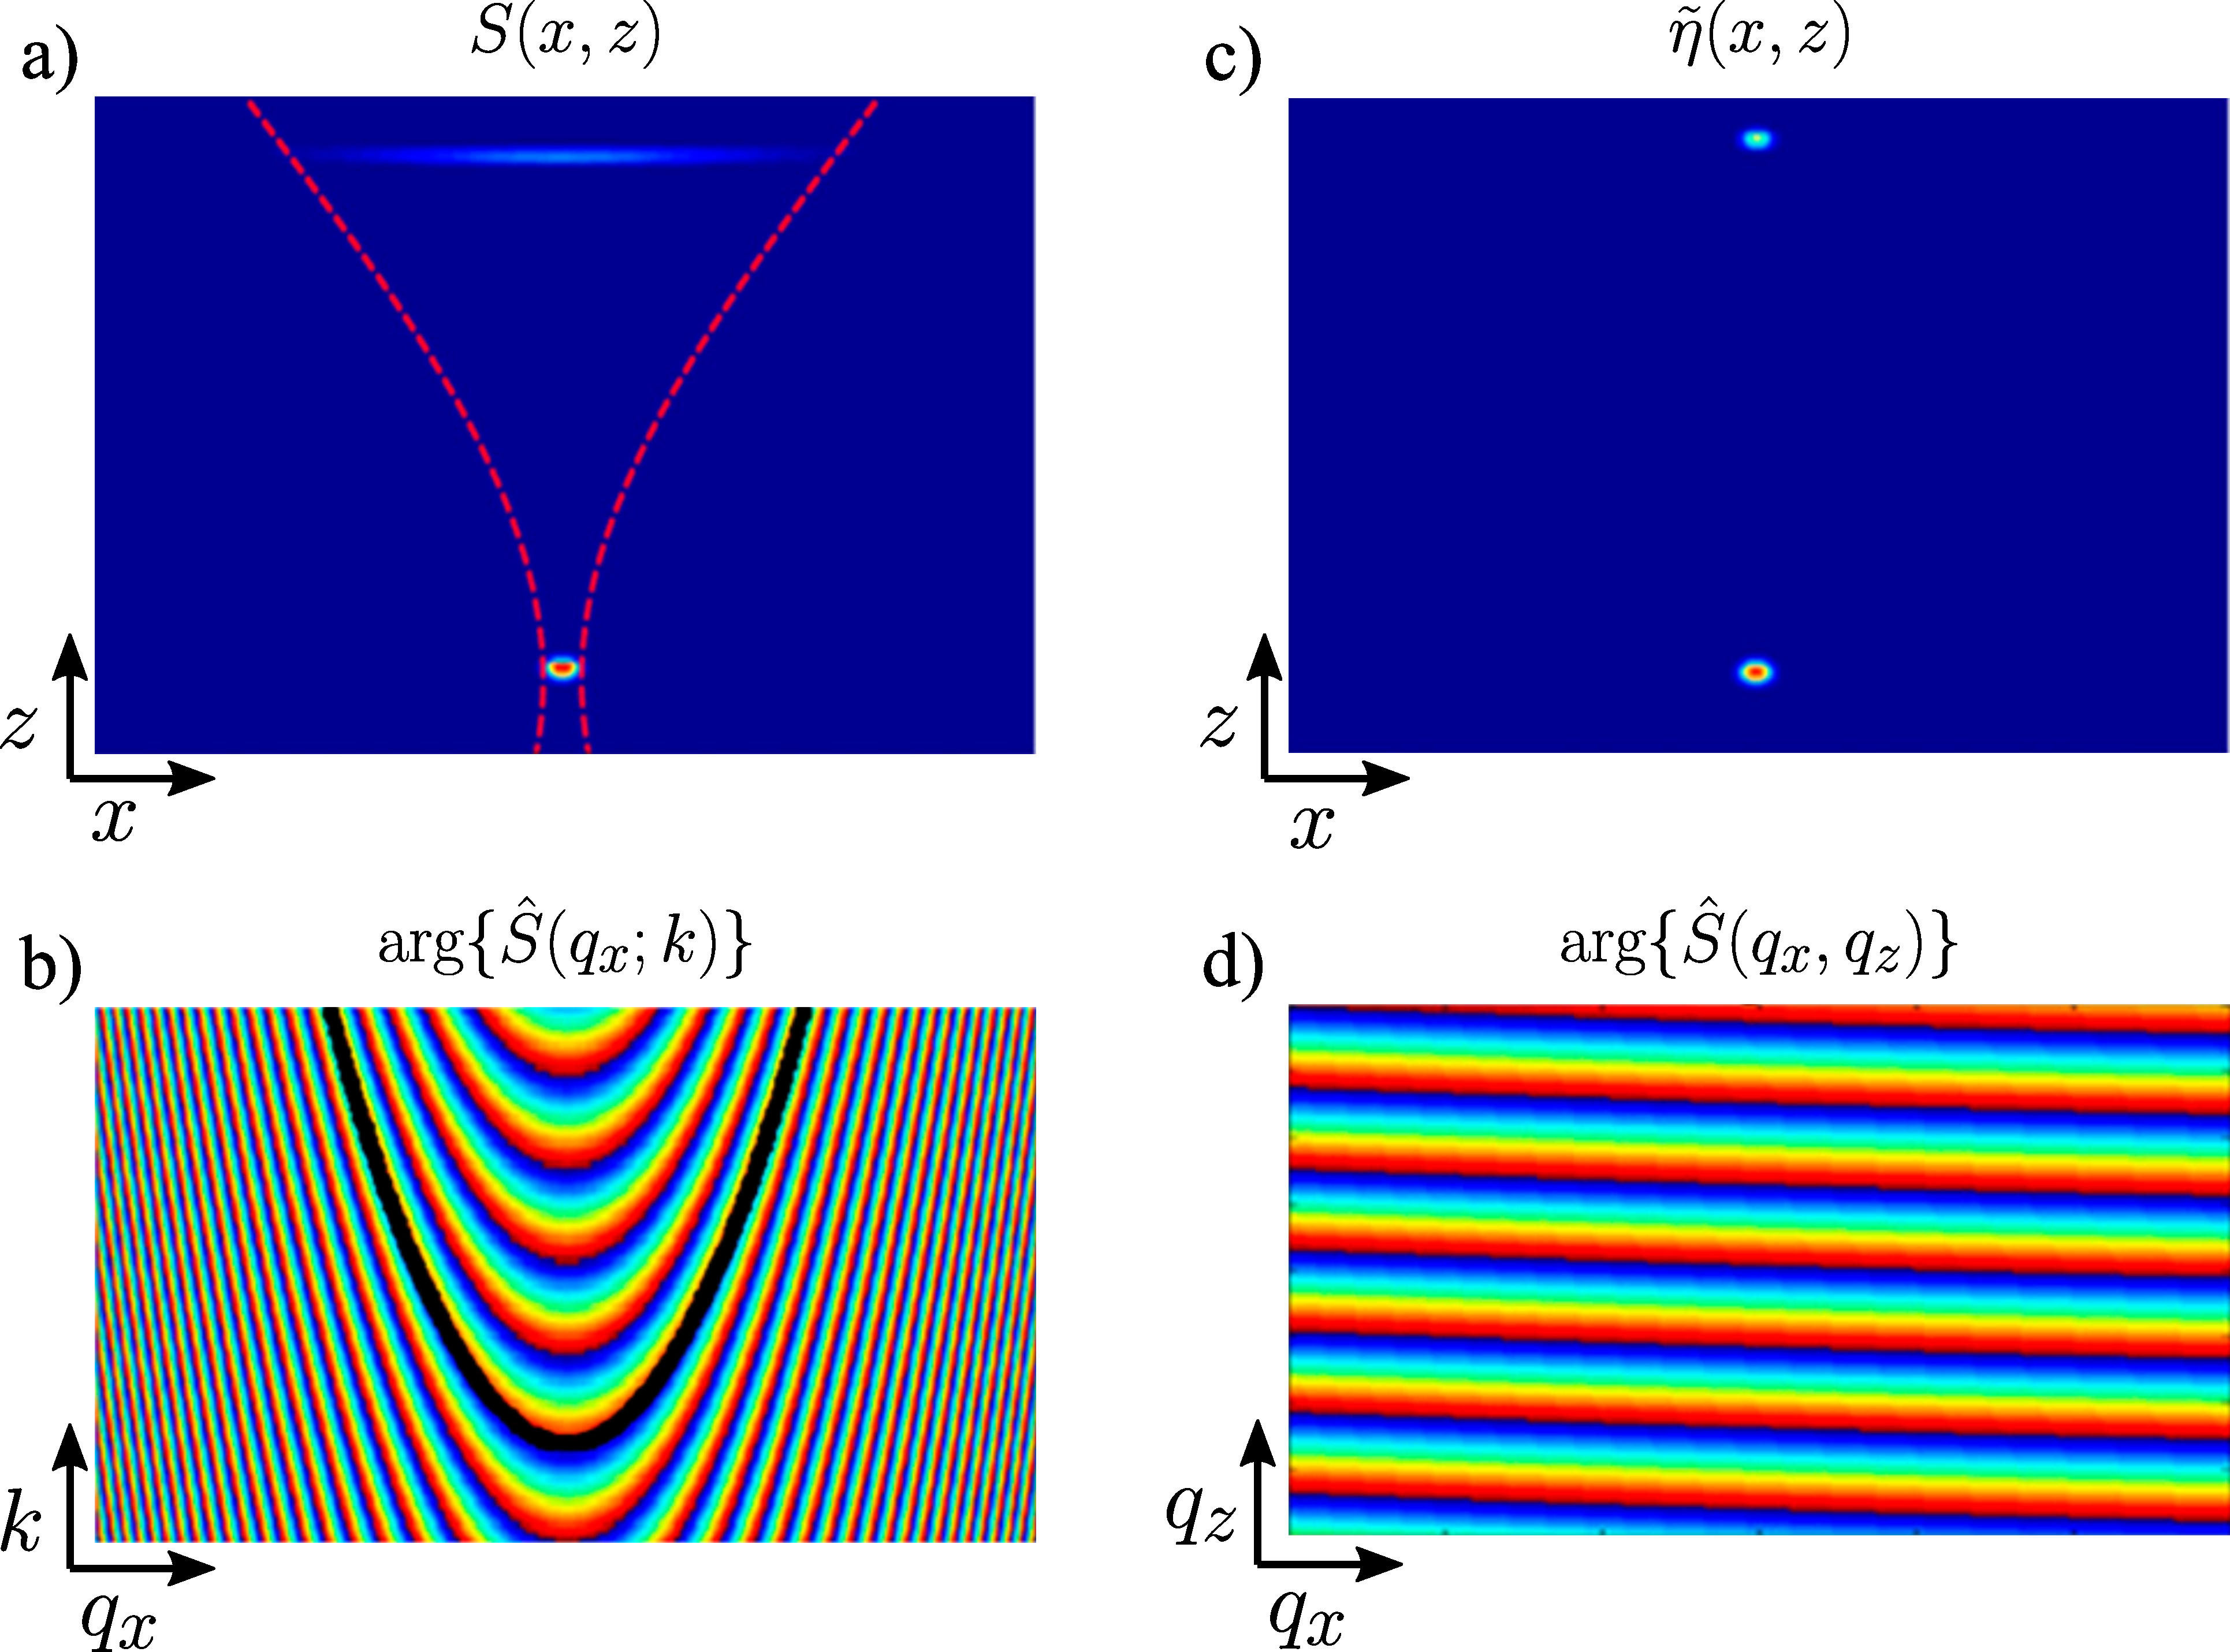
\includegraphics[width=.75\textwidth]{Figures/TheoreticalBasis/ISAM.pdf}
    \caption[Illustration of ISAM operation.]{Illustration of ISAM operation. (a) Acquired B-scan image, (b) phase map of its Fourier transform in $k$-space and (d) in $q_z$-space after re-sampling, yielding ISAM reconstruction in (c). Red line in (a) represents the distribution of the focused beam when positioned in the central Aline, and black line in figure (b) is an example of ISAM sampling curve. Figure adapted from Ref.~\ref{sudkamp}.}
    \label{fig:ISAM}
\end{figure}
\fi

ISAM, first proposed by Ralston \textit{et al}.~\cite{Ralston2006_Interferometric}, has been used widely in the OCT community specially in high-resolution imaging where DoF is greatly reduced and computational correction of defocus is a key tool to extended the DoF~\cite{Liu2014_Computed, Boppart2015_Computational, Yi2019_Structure, Zysk2015_Intraoperative}, being the signal loss the major constrain. Extensions have been made to different imaging geometries and functional imaging, such as rotationally-scanned ISAM for endoscopic OCT~\cite{Marks2006_Inverse-1, Marks2006_Inverse}, and polarization-sensitive ISAM~\cite{Davis2007_Polarimetric}. Furthermore, the development of ISAM have enable real-time \textit{in vivo} visualization~\cite{Ralston2008_Realtime, Ralston2013_Interferometric, St.Marie2013_Robust}. 

\subsection{Digital refocusing}

ISAM reconstruction brings to focus all depths simultaneously, making use of the 3D frequency content of the tomogram. In relatively low numerical aperture systems (NA $<$ 0.15) the re-sampling curve approximates a linear path which means that frequency content in not spread along depth, hence a 2D correction in the transverse plane determined for each plane $z$ independently is sufficient~\cite{Yasuno2006_Noniterative, South2016_Computed} rather than a 3D correction as in ISAM. To isolate a single plane $z_d$, inverse Fourier transform along $k$ of Eq.\eqref{eq:FMft} is computed and evaluated at $z=z_d$ as
\begin{equation}\label{eq:preDefocus}
    \hat{S}(q_x,q_y; z_d) = \int H(q_x, q_y; k) \int \hat{\eta}(q_x,q_y, z_d) e^{iz\sqrt{4k^2-\mathbf{q}^2}} e^{-i2z_dk} \text{d}z\text{d}k.
\end{equation}

Replacing $k=k_c + k'$, being $k'$ the difference between $k$ and central wavenumber $k_c$, the term $(k'/k_c)^2$ is relatively small enough to be neglected, allowing to express $q_z=\sqrt{4k^2-\mathbf{q}^2}$ under the paraxial approximation as~\cite{South2016_Computed}
\begin{equation}\label{eq:qzAprox}
    q_z = 2k_c - \frac{\mathbf{q}^2}{4k_c} + 2k'.
\end{equation}

Replacing $q_z$ in Eq.\eqref{eq:preDefocus}, as well as using convolution theorem to rewrite Fourier integral along $k'$, it is possible to obtain~\cite{South2016_Computed}
\begin{align}\label{eq:preDefocus2}
    \hat{S}(q_x,q_y; z_d) &= \int H(q_x, q_y; k') \int \hat{\eta}(q_x,q_y, z_d) e^{iz(2k_c - \mathbf{q}^2/4k_c + 2k')} e^{-i2z_d(k_c+k')} \text{d}z\text{d}k' \nonumber \\
    &= \int H(q_x, q_y; k') \int \hat{\eta}(q_x,q_y, z_d) e^{i2(z-z_d)k_c} e^{-iz\mathbf{q}^2/4k_c} e^{i2(z-z_d)k'} \text{d}z\text{d}k' \nonumber \\
    &= H(q_x, q_y; z_d) \otimes \left[ \int \hat{\eta}(q_x,q_y, z_d) e^{i2(z-z_d)k_c} e^{-iz\mathbf{q}^2/4k_c}  \delta(2z-2z_d) \text{d}z\right] \nonumber \\
    &= H(q_x, q_y; z_d) \otimes \left[ \hat{\eta}(q_x,q_y, z_d) e^{-iz_d\mathbf{q}^2/4k_c}  \right],
\end{align}
where the convolution is performed along axial axis. The depth-dependent part of $H(q_x,q_y;z_d)$ is related to the axial PSF that can be approximated to a delta function, so that $H(q_x, q_y; z) \propto H(q_x, q_y)\delta(z-z_d)$, which can be replaced in Eq.~\eqref{eq:preDefocus2} to obtain its inverse Fourier transform along $\mathbf{q}$ as
\begin{equation}\label{eq:defocus}
    S(x, y; z_d) = \text{FT}^{-1}_{q_x, q_y}\left\{H(q_x, q_y)\hat{\eta}(q_x, q_y; z_d) e^{-iz_d\mathbf{q}^2/4k_c}\right\}.
\end{equation}

Eq.~\eqref{eq:defocus} is an expression with a form widely known in digital refocusing methods based on scalar diffraction models~\cite{Ralston2005_Deconvolution, Yu2007_Improved, Liu2009_Deconvolution} such as the Fresnel propagator~\cite{Yasuno2006_Noniterative}, where the exponential term is a quadratic phase term responsible of depth-varying defocus. A straightforward inversion of Eq.~\eqref{eq:defocus} provides an approximate refocused sample scattering potential by~\cite{South2016_Computed}
\begin{equation}\label{eq:refocus}
    \tilde{\eta}(x,y; z_d) = \text{FT}^{-1}_{q_x, q_y}\left\{H(q_x, q_y)\hat{S}(q_x, q_y; z_d) e^{iz_d\mathbf{q}^2/4k_c}\right\}.
\end{equation}

Similarly to ISAM, an ideal Gaussian beam can be assumed and $H$ is set to unity. Reconstruction using digital refocusing of Eq.\eqref{eq:refocus} is not complex and implementation is rather simple compared to ISAM, but there are conceptual differences with ISAM reconstruction. In digital refocusing, each depth is brought to focus independently, applying an appropriate quadratic phase term, whereas ISAM reconstruction restores the entire volume simultaneously re-sampling the signal in Fourier domain. More importantly, due to the paraxial approximation in Eq.\eqref{eq:qzAprox}, digital refocusing methods are valid only for low-NA regimes, where there is not coordinates warping that mixes lateral and axial information. Digital refocusing is illustrated in Figure~\ref{fig:IM2} for the low-NA case of the simulated data in Fig.\ref{fig:FM2}, and note that digital refocused image of Fig.~\ref{fig:IM2}(c) exhibit diffraction-limited resolution throughout all depth.

\begin{figure}[htb!]
    \centering
    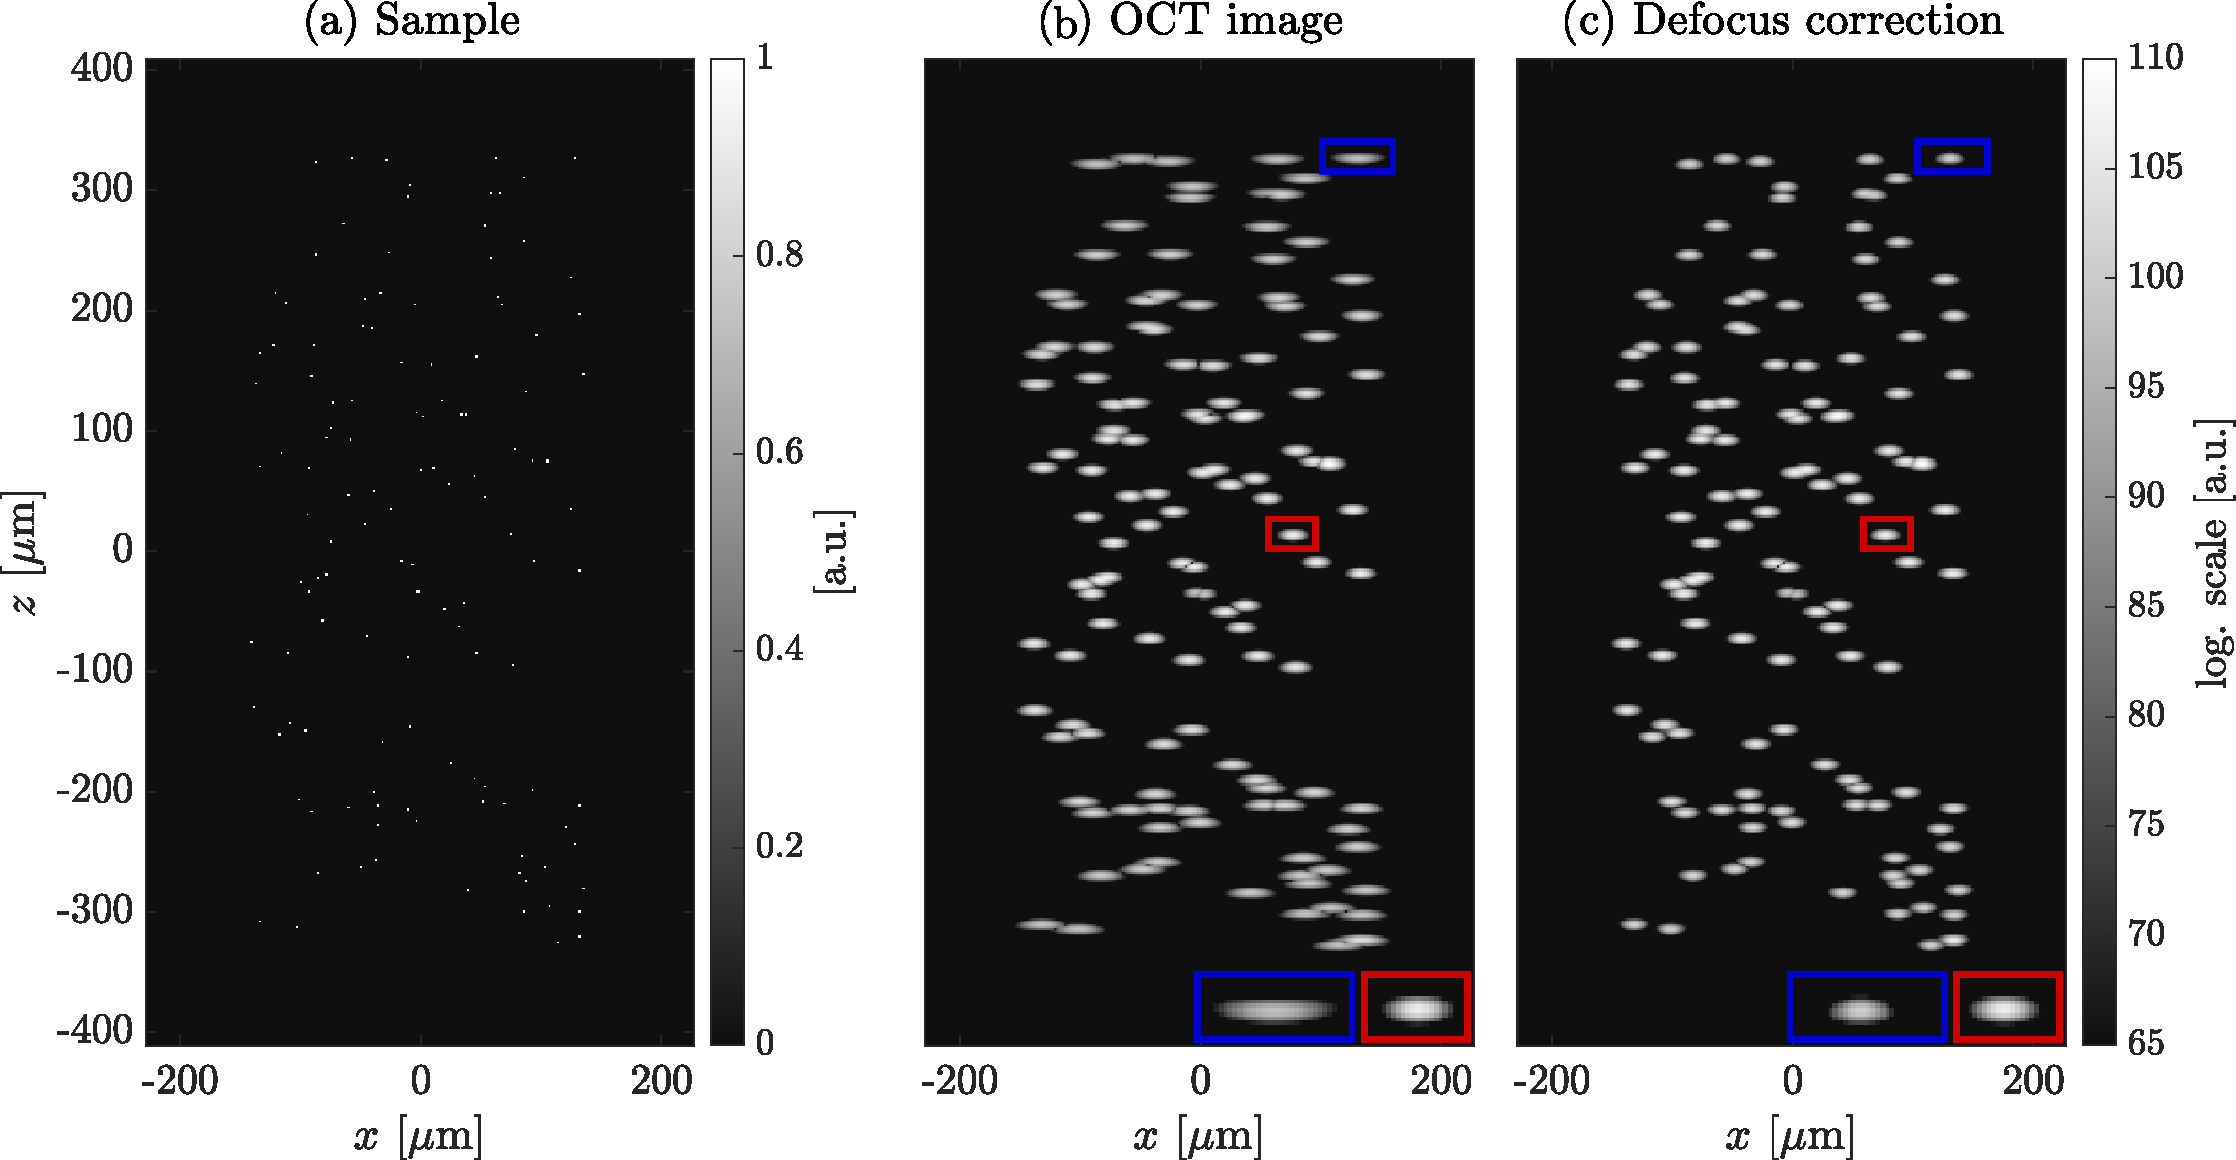
\includegraphics[width=\textwidth]{Figures/TheoreticalBasis/IM_Refocus.pdf}
    \caption[Illustration of digital refocusing.]{Illustration of digital refocusing. (a) Sample consisting of randomly located point scatterers, (b) OCT image simulated using the forward model, (c) digital refocused. (b) and (c) are displayed in logarithmic scale.}
    \label{fig:IM2}
\end{figure}

\subsection{Computational adaptive optics}\label{sec:CAO}

Aberrations are wavefront distortions with respect to a reference wavefront, affecting image quality in imaging techniques such as OCT~\cite{Pircher2017_Review}. Several applications in OCT have benefited from aberration correction, whether using specific optical systems~\cite{Meemon2008_Optical, Xi2009_Highresolution,Mo2013_FocusExtension, Bo2017_Depthoffocus}, hardware-based adaptive optics~\cite{Zawadzki2005_Adaptiveoptics, Zhang2006_Highspeed} or computational adaptive optics~\cite{Kumar2017_Invivo, Hillmann2016_Aberrationfree, Fechtig2014_Line, Wu2019_Computed}. For instance, in retinal imaging, the probe beam is focused onto the retina using the optical system of the eye itself (cornea/lens) that may produce a distorted wavefront affecting image quality~\cite{Liang1997_Aberrations}. In particular, the wavefront in high NA systems is more susceptible to be distorted by imperfections of the optical systems or even the sample itself.

Defocus introduced in the propagation of light is intrinsic to the Gaussian probe beam, for this reason, it is not considered as an optical aberration; in this case aberrations are wavefront deviations from the ideal wavefront of a Gaussian beam. This can be noted in Eq.\eqref{eq:FMft}, where defocus arises from the exponential term whereas wavefront distortions can be modelled by $H(q_x, q_y; k)$ that is related to the effective generalized pupil of the optical system~\cite{Liu2017_Computational}, resulting from the convolution of the illumination and detection generalized pupils, that are identical in OCT given the double-pass geometry.

Recalling the forward model in frequency domain, it is possible to invert Eq.\eqref{eq:preISAM} to obtain an aberration-corrected OCT signal as
\begin{equation}\label{eq:preCAO}
    \tildehat{S}(q_x, q_y; k) = H^{-1}(q_x, q_y; k) \hat{S}(q_x, q_y; k),
\end{equation}
where $H^{-1}(q_x, q_y; k)$ acts as a frequency filter, which depends on spectral and spatial frequency domains, therefore it can address chromatic aberrations~\cite{Liu2017_Computational}. Given the relatively narrow spectrum of the light sources used in OCT, in practical scenarios it is convenient to assume a $k$-independent filter $H(q_x,q_y)$, which is the same for all depths~\cite{Liu2017_Computational}. In hardware-based adaptive optics (AO), the correction filter $H^{-1}(q_x,q_y)$ is applied directly \textit{in situ} to compensate for the distortions of the Gaussian beam~\cite{Zawadzki2005_Adaptiveoptics}, but, because coordinate re-sampling is not included in this correction, $\tilde{S}(q_x, q_y; k)$ is an aberration-corrected signal rather than the sample scattering potential, it means that defocus will be present yet in the acquired images. To correct for defocus using AO, a depth-dependent phase filter is necessary but it is not possible with current hardware such as deformable mirrors. In the case of computational adaptive optics (CAO), the filter is applied in post-processing~\cite{Adie2012_Computational}, enabling the combination of CAO with ISAM or digital refocusing to obtain aberration-free images with focal resolution throughout all depths, namely $\tilde{\eta}(x, y, z)$~\cite{Adie2012_Broadband}. In ISAM reconstruction, $H^{-1}(q_x, q_y; k)$ is already included in Eq.\eqref{eq:ISAM} because $\tildehat{S}(q_x, q_y; k)$ is written explicit in Eq.\eqref{eq:ISAM}. For low-NA regime, the depth-invariant filter $H(q_x,q_y)$ can be generalized in Eq.\eqref{eq:refocus} to a depth-dependent filter $H(q_x,q_y; z_d)$ that includes the exponential term, resulting in~\cite{Adie2012_Computational, Liu2017_Computational} 
\begin{equation}\label{eq:CAO}
    \tilde{\eta}(x, y; z) = \text{FT}_{q_x,q_y}^{-1}\left\{H^{-1}(q_x, q_y; z) \hat{S}(q_x, q_y; z)\right\}.
\end{equation}

In this case, defocus in treated as an aberration contained in the correction filter. The term $H(q_x, q_y; z) = \Omega(q_x,q_z;z) e^{i\varphi(q_x, q_y; z)}$ is a complex filter comprising an amplitude factor $\Omega(q_x,q_z;z)$ and a phase factor $e^{i\varphi(q_x, q_y; z)}$. Phase factor is explicit in Eq.\eqref{eq:refocus} as $e^{iz_d\mathbf{q}^2/4k_c}$ but the idea of CAO is to adaptively defined the phase factor based on the data rather than using the analytical expression~\cite{Adie2012_Computational}, which only accounts for defocus and requires precise knowledge of physical quantities of the system, for instance, the location of the focal plane in the tomogram. The procedure to obtain an aberration-correction sample scattering potential using Eq.\eqref{eq:CAO} is rather simple (note that it is a spatial deconvolution performed in Fourier domain), the key point is to determine the appropriate correction filter. In CAO, the amplitude factor $\Omega(q_x,q_z;z)$ is usually set to unity, because it does not produce a significant impact in image distortions, and a phase-only filter $H(q_x,q_y)=e^{-i\tilde{\varphi}(q_x, q_y; z)}$ is used, where the approximate phase $\tilde{\varphi}(q_x, q_y; z)$ is described in terms of a polynomial basis, such as Zernike polynomials $Z_i$ which are a convention for the description of optical aberrations~\cite{Malacara2007_Optical, Lakshminarayanan2011_Zernike}. Using a weighted sum with $N$ Zernike polynomials, $\tilde{\varphi}(q_x, q_y; z)$ is expressed as
\begin{equation}\label{eq:PhaseDecomp}
	\tilde{\varphi}(q_x, q_y; z) = \sum_i^N Z_i\alpha_i(z_d),
\end{equation} 
with weights $\alpha_i(z)$ that vary with depth. To determine $\alpha_i(z)$, there are two general approaches, optimization-based~\cite{Adie2012_Computational} and sub-apertures correlation~\cite{Kumar2013_Subaperture}.

Sub-apertures correlation method proposed by Kumar \textit{et al}. consists in measuring the local slope of the wavefront in the pupil/Fourier plane to determine the correction phase, emulating a Shack-Hartmann sensor~\cite{Kumar2013_Subaperture}. To do so, the Fourier transform of the acquired signal for each depth, namely $\hat{S}(q_x, q_y; z)$, is split into sub-apertures and the inverse Fourier transform of each sub-aperture is computed to yield images that will exhibit lower resolution and relative shifts between them. These image are cross-correlated to the image of a reference sub-aperture to measure the relative shifts, that is related to the local slope of the wavefront. Then, the local slopes are used to construct the phase correction, possibly using a decomposition like Eq.\eqref{eq:PhaseDecomp}. The number of sub-apertures determines the degree of aberrations that can be corrected. For instance, splitting the pupil into two vertical and horizontal apertures enables defocus correction along the two scan axis. A large number of sub-apertures is desired to be able to correct for high-order aberrations, however, this leads to a significant resolution loss and increased image correlation error, which ultimately results in high errors in the determination of the correction phase.

Optimization-based CAO proposed by Addie \textit{et al}.~\cite{Adie2012_Computational} consists in finding the set of weights $\alpha_i(z_d)$ that improves image quality as measured by a metric via optimization. The iterative operation of this procedure may increase computational time compared to sub-aperture based CAO, but it allows to straightforwardly include high-order aberrations by increasing the number of polynomials and weights used in the correction phase composition. Optimization-based CAO relies on the definition of a proper image quality metric, that ideally must have a minimum (or a maximum) when image aberrations are well compensated, being image sharpness metrics most used for this purpose since aberrations correction is supposed to improve sharpness.

For the following definition of image sharpness metrics, and in subsequent models presented in this work, discrete indexes ($m, n, l$) are used as discrete counterparts of continuous coordinates $(x,y,z)$, respectively. For instance, $S(m,n,l)$ ---sometimes written as $S_{m,n,l}$ for simplicity--- is the discrete counterpart of the ideally continuous signal $S(x,y,z)$. In general, mathematical models will be described in continuous notation, and discrete notation will be used exclusively in equations that are intrinsically discrete.

Shannon's entropy metric $\text{SE}(I)$ of an image $I_{m,n}$ with discrete indexes $(m,n)$ and size $M\times N$ is known to be minimal when aberrations are minimized, it has been used in the context of CAO in OCT~\cite{Hillmann2016_Aberrationfree}, brought from SAR imaging~\cite{Flores1992_Robust}, and is given by
\begin{equation}\label{eq:SE}
	\text{SE}(I) = \sum_i^M\sum_j^N \Gamma(\bar{I}_{i,j}),
\end{equation}
where $\Gamma(I) = -I\log I$, although different transformations can be used, and
\begin{equation}
	\bar{I} = \left|\frac{I}{\sum_i^M\sum_j^N \left|I_{i,j}\right|}\right|^2
\end{equation}
is a normalized intensity image. Here, $I_{m.n}=S_{m,n,l}$ is the current $l$-th \textit{en face} plane being compensated [recall that $S_{m,n,l}$ refers to the discrete version of $S(x,y,z)$].

There are several image quality metrics that have been used in the context of other imaging modalities such as digital holography~\cite{Trujillo2015_Comparative}. For instance, Tamura's coefficient $T = \sqrt{\frac{\sigma(I)}{\left<I\right>}}$ is a measure of contrast~\cite{Memmolo2011_Automatic}, where $\sigma(\cdot)$ is the standard deviation and $\left<\cdot\right>$ is the average value, and gradient-based metrics such as
\begin{equation}
	\text{G(I)} = \sum_i^M\sum_j^N \sqrt{\left[I_{i,j}-I_{i-1,j}\right] ^2 + \left[I_{i,j}-I_{i,j-1}\right] ^2},
\end{equation}
where $I_{m,n} = |S_{m,n,l}| ^ 2$. Image spatial frequency content metrics have been used in sensorless hardware AO and eventually in CAO~\cite{Debarre2007_Image}, and are based on the fact that mid- to high-frequency content of the complex amplitude should increase as resolution improves, i.e. when aberrations are minimized. One possible estimation is the ratio of energy within a band-pass frequency range to the total energy~\cite{Adie2012_Computational}, expressed as
\begin{equation}
	\text{F}(I) = \frac{\sum_i^M\sum_j^N |I_{i,j}B_{i,j}|^2 }{\sum_i^M\sum_j^N |I_{i,j}|^2},
\end{equation}
where $I_{m,n} = \hat{S}_{q_m, q_n,l}$, being $(q_m, q_n)$ discrete counterparts of $(q_x, q_y)$, and $B_{m,n}$ is a band-pass filter with cut-off frequencies tuned to obtain a good performance.

Figure~\ref{fig:CAO} illustrates the effect of aberrations in a simulated \textit{en face} ($xy$ plane) OCT image that was generated elsewhere~\cite{Cuartas-Velez2017_Formacion} with a probe beam waist diameter of $10~\mu$m. The tomogram consists of a large number of point scatterers distributed in the entire field of view as occurs in tissues, with similar index of refraction, producing speckle. In addition, point scatterers with a different index of refraction were added and arranged in a cylindrical shape along horizontal axis $x$, appearing as bright rectangles in the cross-sectional \textit{en face} view of Fig.\ref{fig:CAO}(a) located at the focal plane. Eq.\eqref{eq:defocus} was used to induce defocus as if the \textit{en face} plane of Fig.\ref{fig:CAO}(a) were located at $z=200~\mu$m from the focal plane, and defining the phase of $H$ shown in Fig.\ref{fig:CAO}(e), using Zernike polynomials $Z_5$ and $Z_7$ to induced astigmatism and coma aberrations with random magnitudes, resulting in the aberrated \textit{en face} of Fig.\ref{fig:CAO}(b), where blurring is evident and consequently resolution loss.

\begin{figure}[htb!]
	\centering
	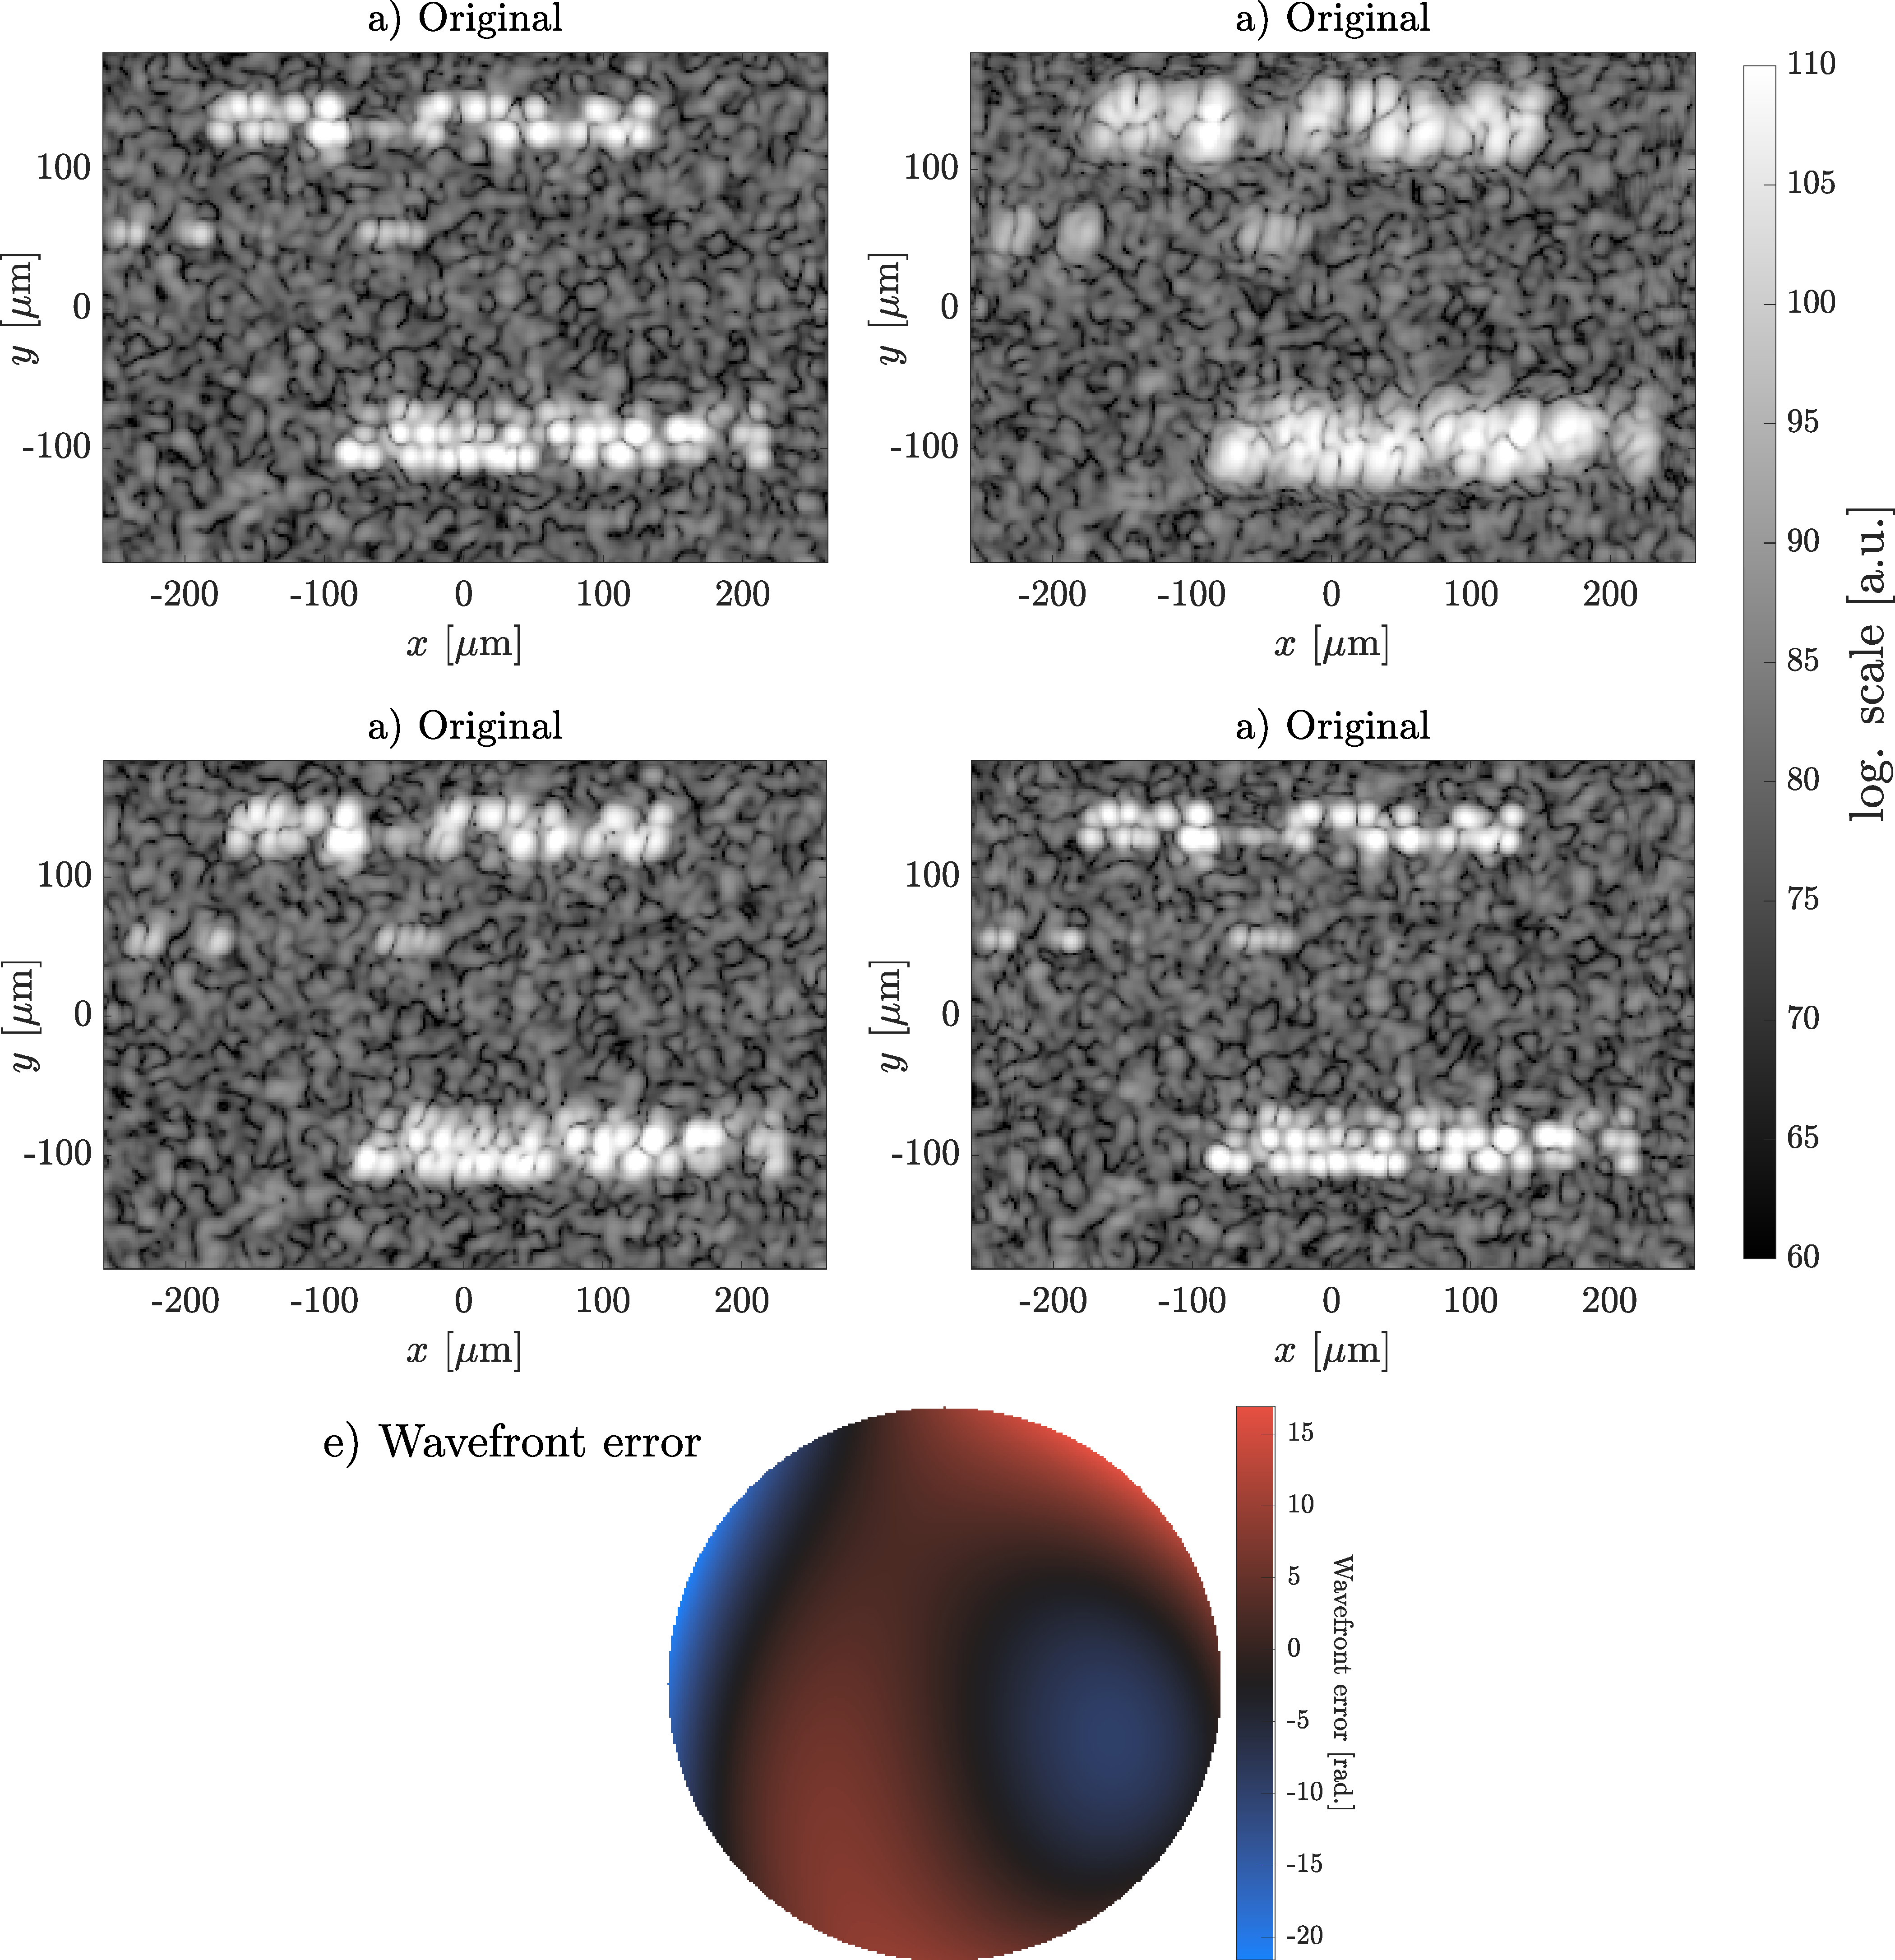
\includegraphics[width=\textwidth]{Figures/TheoreticalBasis/CAO.pdf}
	\caption[Illustration of computational adaptive optics.]{Illustration of computational adaptive optics. Simulated OCT \textit{en face} image (a) without and (b) with aberrations and defocus, induced using the wavefront in (e). Result of (c) digital refocusing and (d) computational adaptive optics. (a)--(d) are displayed in logarithm scale.}
	\label{fig:CAO}
\end{figure}

Digital refocusing was applied to the aberrated \textit{en face} using Eq.\eqref{eq:refocus} setting $H=1$, resulting in a refocused image with partial resolution improvement due to the presence of the remaining two aberrations deteriorating image quality. On the other hand, optimization-based CAO was applied to the aberrated \textit{en face} using Eq.\eqref{eq:CAO}, describing the phase correction filter with $Z_4$, $Z_5$ and $Z_7$, being $Z_4$ Zernike polynomial for defocus. Aberration-corrected \textit{en face} view of Fig.\ref{fig:CAO}(d) exhibits focal resolution similar to the original \textit{en face}, demonstrating the possibility of correcting defocus and additional aberrations using CAO.

To illustrate the behavior of image quality metric that is the basis of CAO, original \textit{en face} of Fig.\ref{fig:CAO}(a) was defocused using $Z_4$ weighted by $\alpha_4=17.8$ and then several corrected images were created with weights linearly varying between $[-40, 20]$. Figure~\ref{fig:Sharpness} shows a plot of Shannon's entropy of the corrected image as a function of the correction weight $\tilde{\alpha}_4$, exhibiting a smooth behavior with a clear minimum at nearly $\tilde{\alpha}_4=-17.8$, where the negative sign is because the correction phase term is the conjugate of the actual defocus term. Alongside Shannon's entropy, there are six example \textit{en faces} with different phase corrections, with the optimal \textit{en face} enclosed in a red box, showing the best image quality among them.

\begin{figure}[htb!]
	\centering
	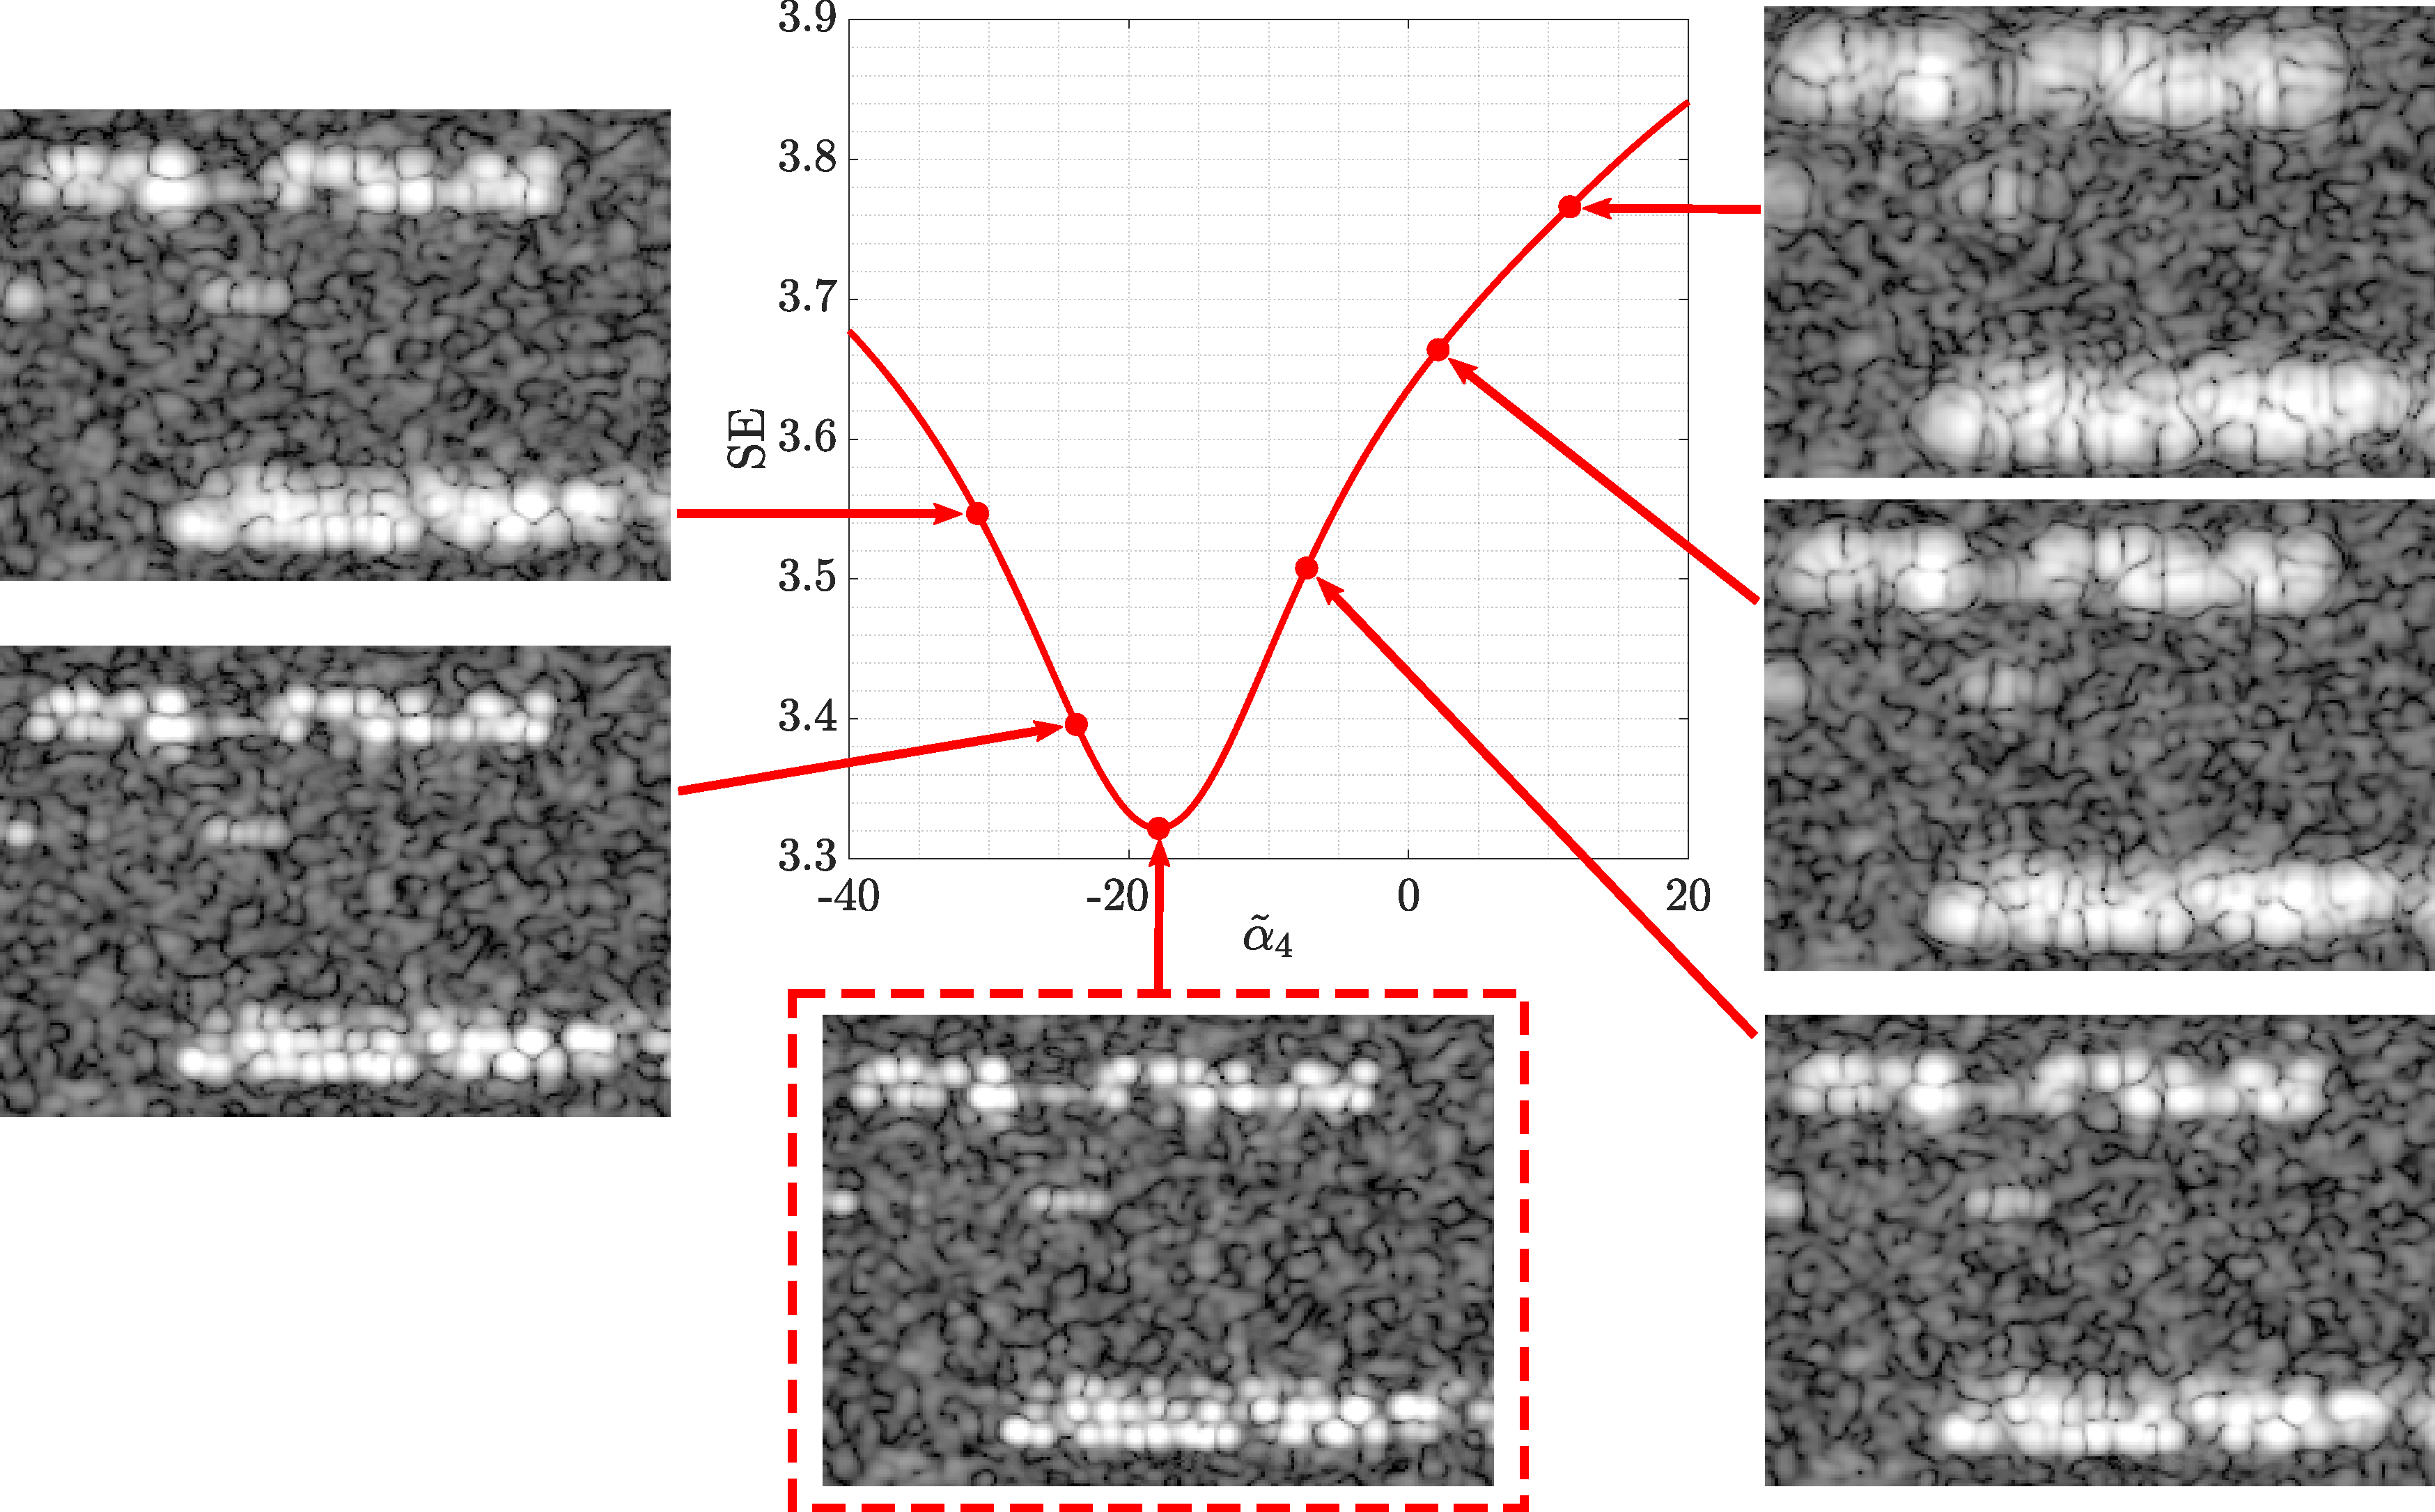
\includegraphics[width=\textwidth]{Figures/TheoreticalBasis/SharpnessCAO.pdf}
	\caption[Illustration of Shannon's entropy metric.]{Illustration of Shannon's entropy metric to measure image sharpness of a defocused \textit{en face} image corrected using Zernike polynomial $Z_4$. Plot shows the value of SE as a function of correction weight $\tilde{\alpha}_4$. Surrounding \textit{en faces} images were corrected with different weights for a visual inspection of image quality. Optimal corrected image (on the red rectangle) corresponds to the minimum value of SE.}
	\label{fig:Sharpness}
\end{figure}

Computational adaptive optics promises to be a powerful alternative to hardware-based adaptive optics that require very complex optical setups, specially in retinal imaging where the demand of cellular imaging increases, for example in photo-receptors mosaic imaging~\cite{Kumar2017_Invivo, Hillmann2016_Aberrationfree, South2018_Combined}.

There are two necessary requirements for computational aberration correction: acquired tomogram should possess phase stability which is so far the major requirement~\cite{Shemonski2014_Stability, Liu2017_Computational, South2016_Computed}, but in addition, the lateral sampling must satisfy Nyquist sampling~\cite{Liu2017_Computational}, i.e. lateral sampling must be equal or smaller than half the beam waist diameter, otherwise high-frequency content is not recovered properly and results will present distortions. In fact, Nyquist sampling is necessary in general for computational refocusing in any imaging technique, not only in OCT~\cite{Wallace2001_Workingpersons, Pawley2006_Handbook, Biggs2010_3D}. 

\FloatBarrier

\subsection{Phase stability requirement} \label{sec:phaseStab}

Computational techniques described previously rely upon accurate measurements of the complex amplitude information in order to guarantee a coherent aperture synthesis, necessary for aberration correction. Complex amplitude comprises amplitude and phase information, but phase is more susceptible to undesired fluctuations~\cite{Vakoc2005_Phaseresolved}, hence reliable phase measurement is not a straightforward task due to experimental constrains as explained in Section~\ref{sec:OCTConfigPhaseStab}. In fact, first digital refocusing approaches in OCT were based on the intensity~\cite{Ralston2005_Deconvolution, Woolliams2010_Spatially, Liu2009_Deconvolution}, but they provided very limited results given that incoherent deconvolution ignores the phase information. Such initial approaches were designed to work with the intensity signal possibly because of the lack of phase-stable measurements in early OCT systems.

The aim of this section is to discus phase stability requirement in the context of computational aberration correction. Phase stability is affected by phase noise that may arise from the system or the sample. System-induced phase noises, such as phase-jitter~\cite{Vakoc2005_Phaseresolved} and galvanometer-induced phase noise~\cite{Adie2015_Interferometric, White2003_vivo}, were explained in Section~\ref{sec:OCTConfigPhaseStab}. On the other hand, sample-induced phase noise arises from sample motion~\cite{Shemonski2014_Stability-1}, therefore it affects mainly \textit{in vivo} imaging which is more prone to motion during signal acquisition than \textit{ex vivo} imaging. Motion can be either global, such as involuntary motion of the subject, or internal, such as blood flow in arteries.

Development of computational aberration correction has been grounded in SDOCT systems. For this reason, most significant phase instabilities induced by the system arise from the galvanometer scanners, which can be experimentally avoided in some cases, therefore, in this area, major attention have been put in sample motion-induced phase noise, which is the focus of following discussions.

Sample motion have two primary effects in the complex OCT signal; effective shift of the complex amplitude and phase-only jump~\cite{Chen1997_Optical, White2003_vivo, Shemonski2014_Stability}. The former effect is rather intuitive, it is the displacement of apparent location of the signal in the tomogram, affecting both amplitude and phase. The latter effect is an additional phase-only jump that is a consequence of Doppler effect, and actually it is used for functional imaging techniques like flowmetry~\cite{Braaf2019_OCTBased}. Both effects have an impact in the phase of the tomogram and therefore they affect phase stability, but their individual influence vary depending on system parameters~\cite{Shemonski2014_Stability}. Effective complex amplitude shift scales with the spatial resolution of the system; system with fine resolution may be more susceptible to motion artifacts. In general, axial resolution is finer than lateral resolution, therefore this effect have a greater impact in the axial direction. On the other hand, phase-only jump $\delta$ is a consequence of motion in the axial direction only, and is proportional to the axial displacement $\delta z$ and the central wavenumber, $\delta = 2k_c\delta z$, where the factor of two is due to the double-pass, reflection geometry. Since $k$ is typically a relatively large value (of the order of $10^6$) relatively small displacements $\delta z$ can produce significant phase jumps $\delta$, and this is why optical phase-sensitive techniques can measure very small displacement using optical interferometry, but in the case of CAC this is an undesired phase contribution that in general have a greater influence than complex amplitude shift effect. For this reason, in some cases there is not an evident displacement in the tomogram intensity due to motion, yet there may be phase jumps reducing phase stability.

In practical terms, motion artifacts are negligible during one A-line acquisition under controlled circumstances, in the case of SDOCT because of the parallel acquisition in $k$-space, and in SSOCT because of the high A-line acquisition rate. However, motion artifacts may appear during acquisition of multiple A-lines and more significantly during acquisition of multiple B-scans which have a longer repetition time. Complex amplitude shifts appear as relative displacements between A-lines or B-scans, whereas phase-only jumps produce a relative phase offset between A-lines or B-scans. For these reasons, hereafter 1D and 2D phase stability are used to refer to phase stability along one or two lateral scan axes, obviating phase stability along axial direction which in general is ensured.

Figure~\ref{fig:motionEx} illustrates motion artifacts in OCT, using a simulated B-scan generated similarly to that of Fig.\ref{fig:IM2}, except that axial motion was added when computing the $n$-th A-line by changing the position $z$ of all scatters by $z + \delta z_n$, where $\delta z_n$ represents the magnitude of motion, with random values defined for each A-line, inside a predefined range. This corresponds to a rigid body or \textit{bulk} motion because the entire sample is displaced by the same amount in every A-line. The simulated intensity B-scan with a static sample is shown in Fig.\ref{fig:motionEx}(a), displaying defocus away from the focal plane located at $z=0$. This image was re-generated inducing inter-A-line motion randomly distributed with standard deviation $1~\mu$m, shown in Fig.\ref{fig:motionEx}(d), and the resulting intensity B-scan shown in Fig.\ref{fig:motionEx}(b) exhibits spurious relative shifts between A-lines, which in this case are evident because the magnitude of motion is of the order of axial resolution 5~$\mu$m.

\begin{figure}[htb!]
	\centering
	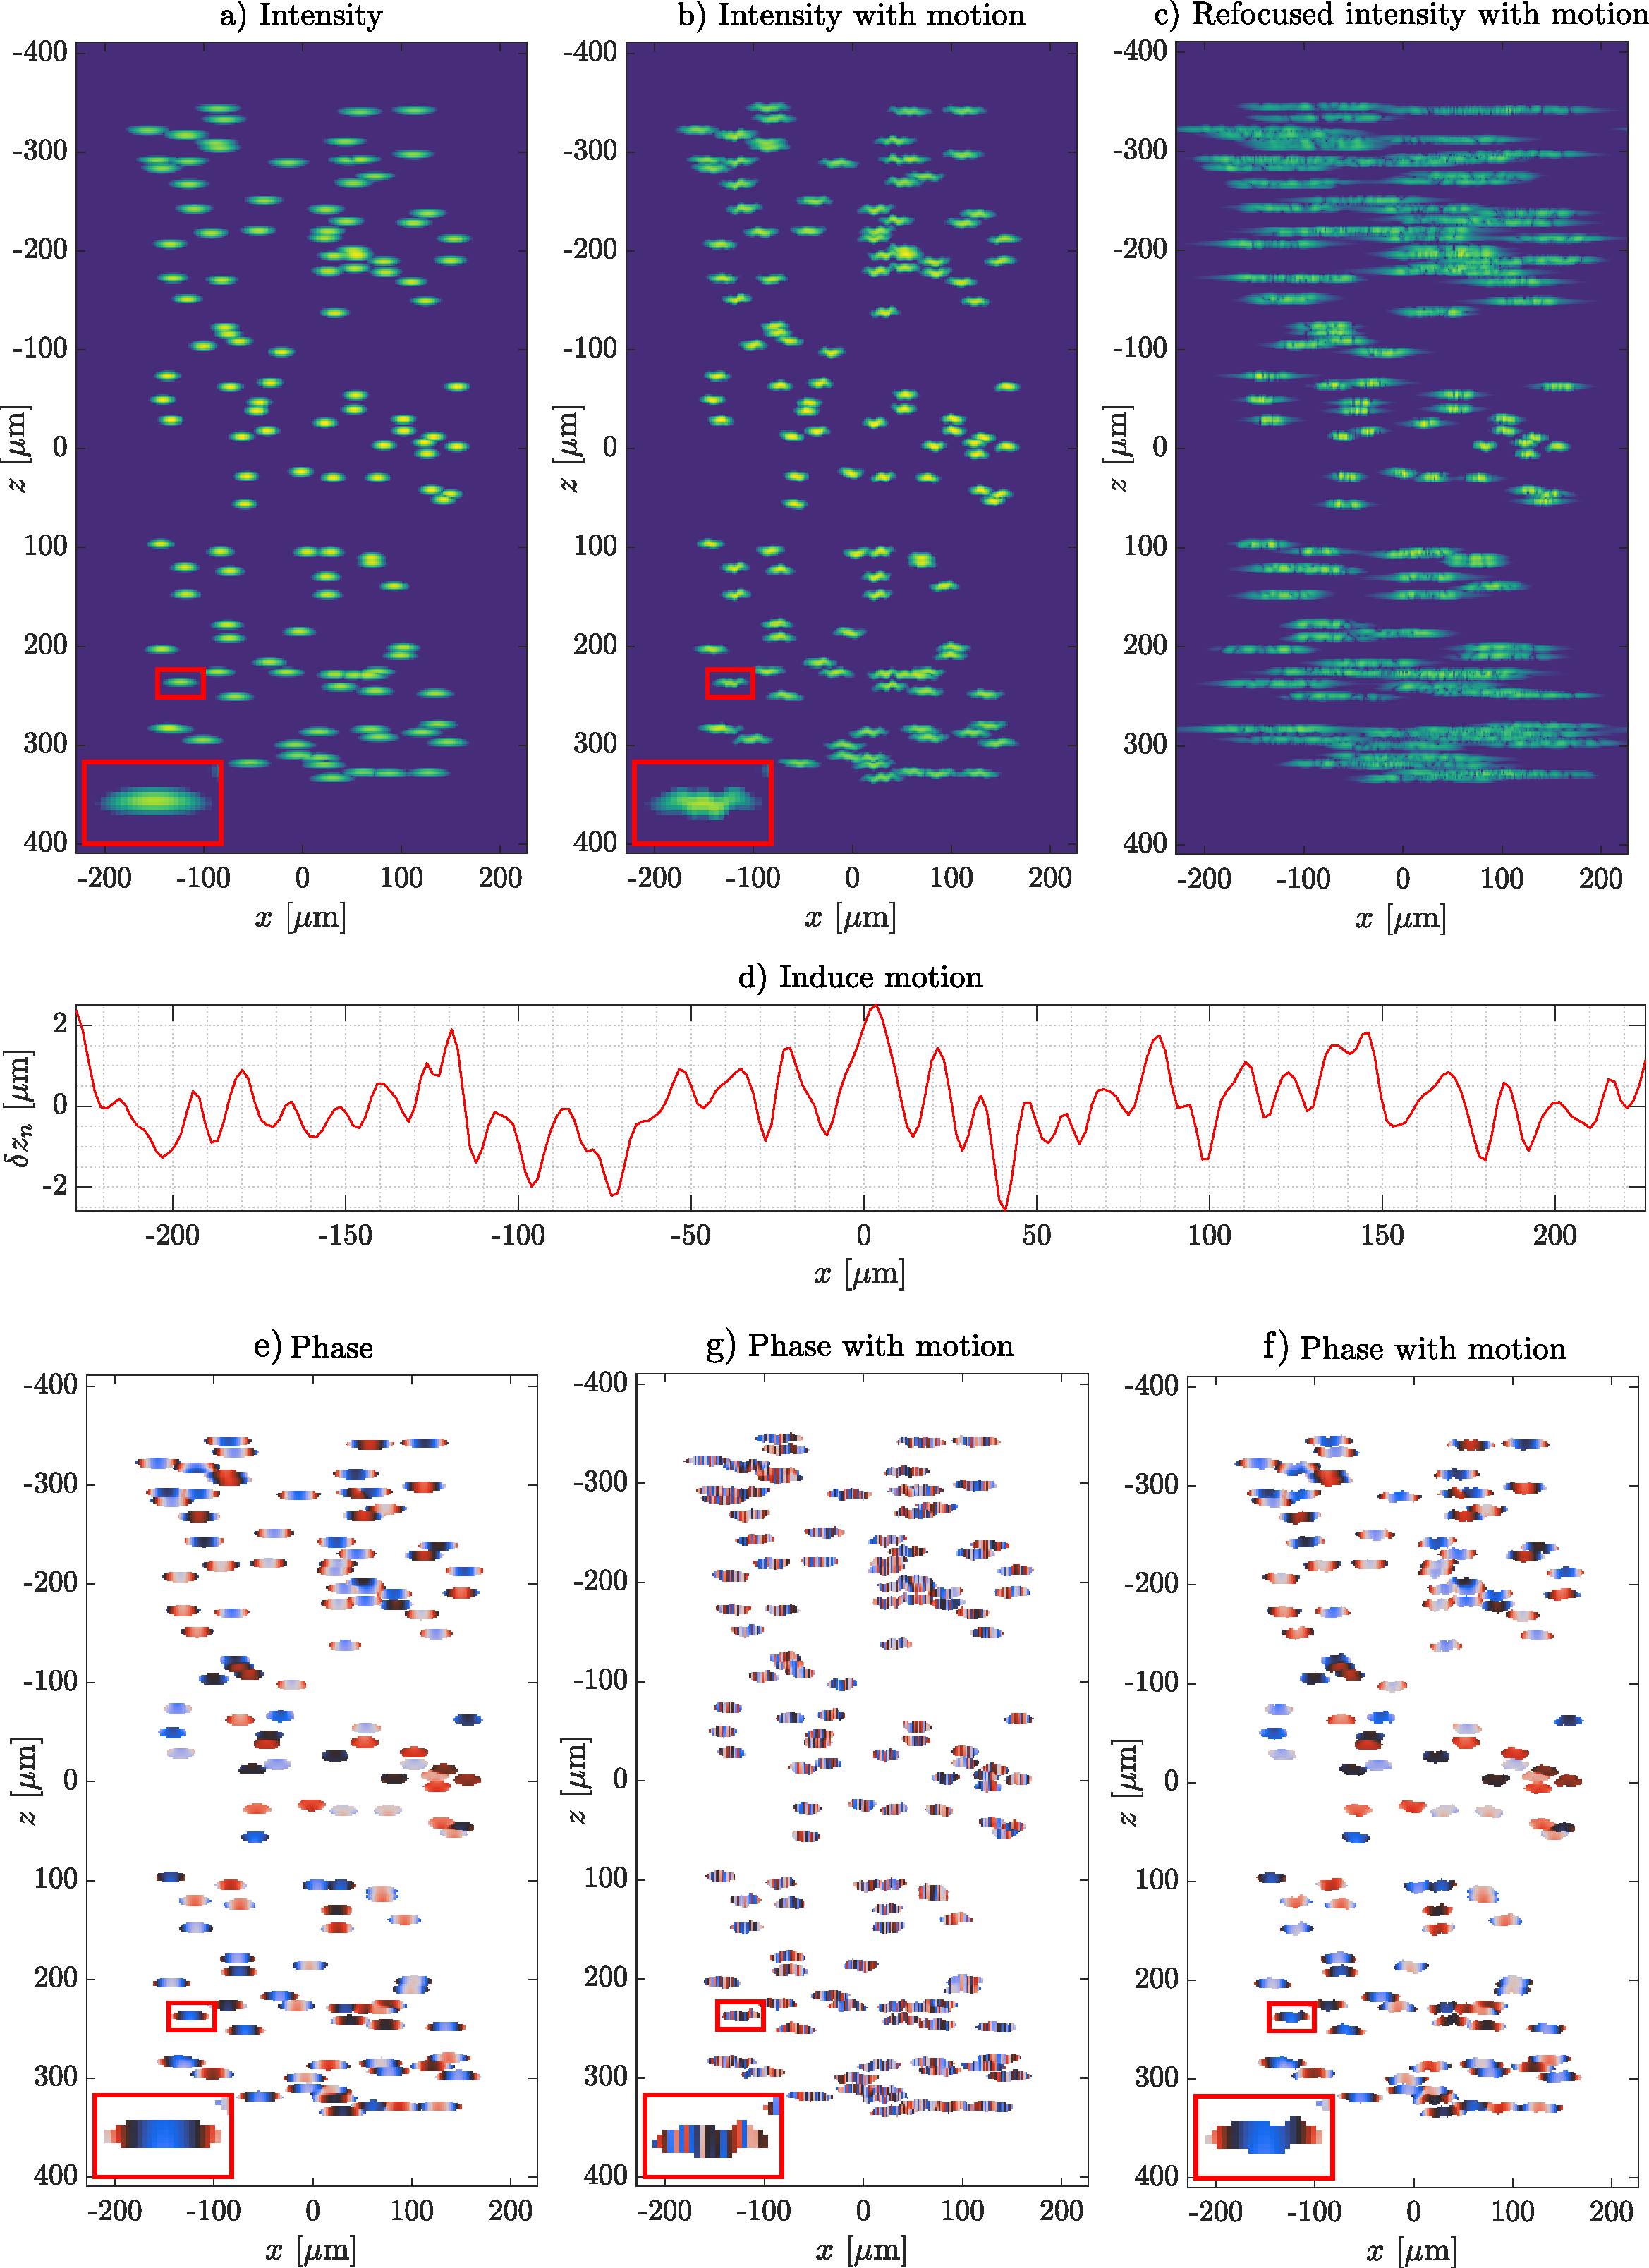
\includegraphics[width=.95\textwidth]{Figures/TheoreticalBasis/MotionEx.pdf}
	\caption[Illustration of the impact of motion in phase stability and digital refocusing.]{Illustration of the impact of motion in phase stability and digital refocusing. OCT image simulated using the forward model, (a) with static sample; (b) with sample motion shown in (d), that results in the unsuccessful digital refocused image in (c). Note the relative shift between A-lines when comparing the insets in red rectangles. Phase images: (a) with static sample; (g) with sample motion shown in (d) and the same of (g) but ignoring the Dopple phase jumps.}
	\label{fig:motionEx}
\end{figure}

\FloatBarrier

To evaluate phase stability, Fig.\ref{fig:motionEx} shows phase images computed as $\arg\{S_{m,n,l}\}$, where a threshold was used to display only regions with high intensity, corresponding to the point scatterers. Fig.\ref{fig:motionEx}(e) is the phase with the static sample, exhibiting a stochastic but smooth behavior, distinctive of phase-stable images, opposed to the phase image after inducing motion shown in Fig.\ref{fig:motionEx}(e) that exhibits very poor phase stability because of the relative shifts between A-lines, also observable in the intensity image in Fig.\ref{fig:motionEx}(b), and more importantly due to the random phase offsets induced by Doppler jumps, not observable in the intensity image in Fig.\ref{fig:motionEx}(b). Lack of phase stability frustrates the operation of digital refocusing or any other phase-dependent aberration correction method, as is evident in Fig.\ref{fig:motionEx}(c). To compare the influence of the two effects of motion, Fig.\ref{fig:motionEx}(f) shows the phase when ignoring the motion-induced phase offsets, thus considering only the complex amplitude shifts, and it can be noted that phase is smoother than that of Fig.\ref{fig:motionEx}(g) affected by both motion artifacts, however, even ignoring phase jumps, in this example complex amplitude shifts alone are strong enough to frustrate any aberration correction.

To quantitatively determine that certain tomogram has sufficient phase stability for a phase-dependent technique to work properly is somehow not possible (unless attempting CAC and then visualizing if results are corrupted or not), instead, it is possible to recognize when phase stability is not enough for such techniques to provide reliable results. Some systematic studies have been carried out to show the effect of various types of motion on defocus correction, namely, 1-D Brownian motion, steps functions and sinusoidal motion, and this helped to determined thresholds for admissible motion magnitudes for successful aberration correction to assist the design of OCT systems, for instance to determine an adequate imaging speed. Such works include simulated studies, as well as experimental studies with \textit{ex vivo} sample~\cite{Shemonski2014_Stability}, and a further extension with \textit{in vivo} imaging~\cite{Shemonski2014_Stability-1}, finding out that in terms of motion-induce phase noise, axial motion plays indeed the most important role in phase stability, although in some experimental scenarios traverse motion may be significant as well.

It is important to recall that phase stability is more difficult to achieve in SSOCT compared to SDOCT given that the former is susceptible to phase-jitter describing a linear depth-dependent noise, in addition to the phase noise sources affecting in SDOCT.

\FloatBarrier

\subsection{Phase stabilization}\label{sec:phaseStabilization}

Given that the presence of phase noise in acquired tomograms is quite difficult to avoid or suppress experimentally~\cite{Adie2015_Interferometric}, phase stabilization in post-processing have been developed for phase-dependent imaging techniques in OCT like aberration correction and Doppler OCT. Phase stabilization techniques were designed to correct for phase jumps between A-lines, whether they arise from sample-motion or the system itself, but they cannot address complex amplitude shifts so that they must be small enough to be considered negligible. In this section, numerical phase stabilization approaches are presented oriented to the correction of phase offsets. In fact, correction of phase offsets is not sufficient for phase-jitter correction which is a linear depth-dependent phase noise, however the methods presented here can be extended to address phase-jitter with slight modification, and the core discussions of this section applies equally for this type of phase noise.

An early phase stabilization approach employs a reference signal consisting in an highly reflective flat surface in the sample arm, like a mirror or even a coverslip~\cite{Ralston2006_Phase, Yang2001_Phasereferenced}. The phase of this reference signal is assumed to be space-invariant, thereby any phase jump between A-lines must be due to phase noise. The procedure consist in identifying and extracting the reference signal in the tomogram $S(m,n,l)$, which should appear across the entire lateral field of view but typically occupy only a small set of pixels $L$ in the axial direction, and in a phase-stable tomogram it should have a constant phase value. Then, the phase difference between adjacent A-lines $m$ and $m-1$ are computed as
\begin{equation}\label{eq:PhaseDiff}
	\delta(m,n) = \arg\left\{\sum_{l\in L} S(m,n,l)S^*(m-1,n,l)\right\},
\end{equation}
where $^*$ denotes complex conjugate and the summation over $L$ is to average the phase of phasors along depth only in the pixels occupied by the reference reflection. Phase differences $\delta(m,n)$ are relative to consecutive A-lines. The absolute phase differences $\Delta(m,n)$ with respect to a reference A-line, typically the first A-line, are calculated using a cumulative sum as
\begin{equation} \label{eq:absPhaseDiff}
	\Delta(m,n) = \sum_{\hat{m}=1}^m \delta(\hat{m},n).
\end{equation}

Finally, the phase-corrected tomogram $\tilde{S}(m,n,l)$ is computed applying the conjugate phase differences,
\begin{equation}
	\tilde{S}(m,n,l) = S(m,n,l)e^{-i\Delta(m,n)}.
\end{equation}

To summarize, this phase stabilization process, refer to as \textit{hardware-based} stabilization, consists in applying a conjugate phase offset that is determined for each A-line using the phase difference between consecutive A-lines considering only a region of the signal containing a reference constant phase. There are some important features to remark. First, the correction phase is depth-independent; it consists of a global phase offset for every A-line, hence it cannot correct for phase-jitter which is a depth-dependent ramp phase noise as noted in Eq.\eqref{eq:phaseJitter}. An extension to cover phase-jitter is possible and has been developed~\cite{Vakoc2005_Phaseresolved} as will be explained later. Second, the need of a reflective surface in the sample arm is difficult to implement in practical terms, specially for \textit{in vivo} imaging where it is not easy to add a mirror in the sample arm directly. A very used approach is to separate the sample arm into two paths, one for the sample and the other for a mirror, but this is based on hardware modifications not present in basic OCT setups. 

This hardware-based phase stabilization approach was crucial for the development of CAC techniques like ISAM in an early stage~\cite{Ralston2006_Phase}. However, this is an unpractical approach because it relies on a hardware modification of the system. Fully numerical approaches were developed in the context of Doppler OCT~\cite{White2003_vivo}, then its use migrated to the field of CAC and are currently in the use~\cite{Shemonski2014_Threedimensional}. Fully numerical approaches rely on the use of the signal information itself to determine the relative phase offset between A-lines using Eq.\eqref{eq:PhaseDiff}, except that the entire axial scan $S(m,n,l)$ is employed instead of using the signal from a reference reflector, and then phase correction of absolute phase offsets is performed similarly to the previous description.

Operation of this method relies on speckle correlation: in phase-stable tomograms, phase difference between consecutive A-lines must approximate to zero if speckle is fully correlated, thus any phase fluctuation is due to phase noise~\cite{White2003_vivo}. Correct speckle sampling is necessary because otherwise phase difference would be due to phase noise but also due to speckle decorrelation, yielding an erroneous phase correction. A correct sampling of speckle is obtained when Nyquist sampling theorem is fulfilled, actually this requirement is already imposed by CAC techniques. This method provides sufficient phase stability for phase-dependent techniques like CAC, but it suffers from some imperfections and thus results are limited.

More specifically, because tissues are not homogeneous as is the case of a reference reflector, there are phase difference associated to changes in the tissue that are insignificant at local level, i.e. in the computation of relative phase differences $\delta(m,n)$, but become significant in the accumulation used to compute the absolute phase differences $\Delta(m,n)$ in Eq.\eqref{eq:absPhaseDiff}. Imperfection also arises when there are noisy A-lines or with no signal at all where phase correction may fail, producing errors that propagates in the cumulative sum, denoted here as \textit{long-range} errors. In other words, this method yields \textit{local} phase stability but the propagation of errors due to the cumulative sum results in long-range errors that frustrate obtaining \textit{global} phase stability. However, this is not a limitation for CAC techniques, because it is known that local phase stability is sufficient to perform the deconvolution operation that is the basis of CAC~\cite{Shemonski2014_Stability}, since the deconvolution kernel in practical scenarios has a relatively small size thus only local information from a small neighborhood of A-lines is merged in the deconvolution, which means that it is sufficient to have local phase stability, at the scale of the deconvolution kernel size.

It is important to remark that phase values that can be corrected are arbitrary despite phase wrapping may appear. Suppose a certain A-line $S_A$ is experimentally phase-shifted by $2\pi r$ with $r\in\mathbb{R}$, resulting in $\tilde{S}_A=S_Ae^{i2\pi r}$. Phase shift $2\pi r$ can be decomposed as $2\pi r = \Delta + 2\pi n$ with $n\in \mathbb{Z}$ and the effective computed phase shift $\Delta$ being in the range $[-\pi, \pi]$. Therefore, shifted A-line is $\tilde{S}_A=S_Ae^{i\Delta} e^{i2\pi n}=S_A e^{i\Delta}$, showing that a phase correction in the range $[-\pi, \pi]$ is sufficient and the $n$ additional cycles of $2\pi$ are inconsequential given that $\tilde{S}_A = \tilde{S}_Ae^{i2\pi n}$. In fact, this discussion in valid in the context of computational aberration correction where the requirement is to maintain a constant phase relation between measurements~\cite{Shemonski2014_Stability}, but in certain applications quantification of phase shifts is necessary thus in such cases phase wrapping must be properly addressed, for instance, for the proper quantification of flow velocity in Doppler OCT~\cite{Hong2012_Highpenetration}.

Examples of phase stabilization are shown in Fig.~\ref{fig:PhaseStabilization} for an OCT B-scan simulated using the forward model for a low NA system as in previous examples. In this case, there are 10000 point scatterers with random positions and equal index of refraction to produce speckle and 128 points with random positions and random index of refraction producing higher intensity than the background scatterers, as can be noted in the intensity image in Fig.~\ref{fig:PhaseStabilization}(a). Bulk sample motion randomly distributed with standard deviation $0.1~\mu$m was added, and such motion do not induce noticeable complex amplitude shifts as can be seen in Fig.~\ref{fig:PhaseStabilization}(a), but phase offsets are strong as shown in the phase image of Fig.~\ref{fig:PhaseStabilization}(b) that presents strong fluctuations that greatly reduce phase stability.

\begin{figure}[htb!]
	\centering
	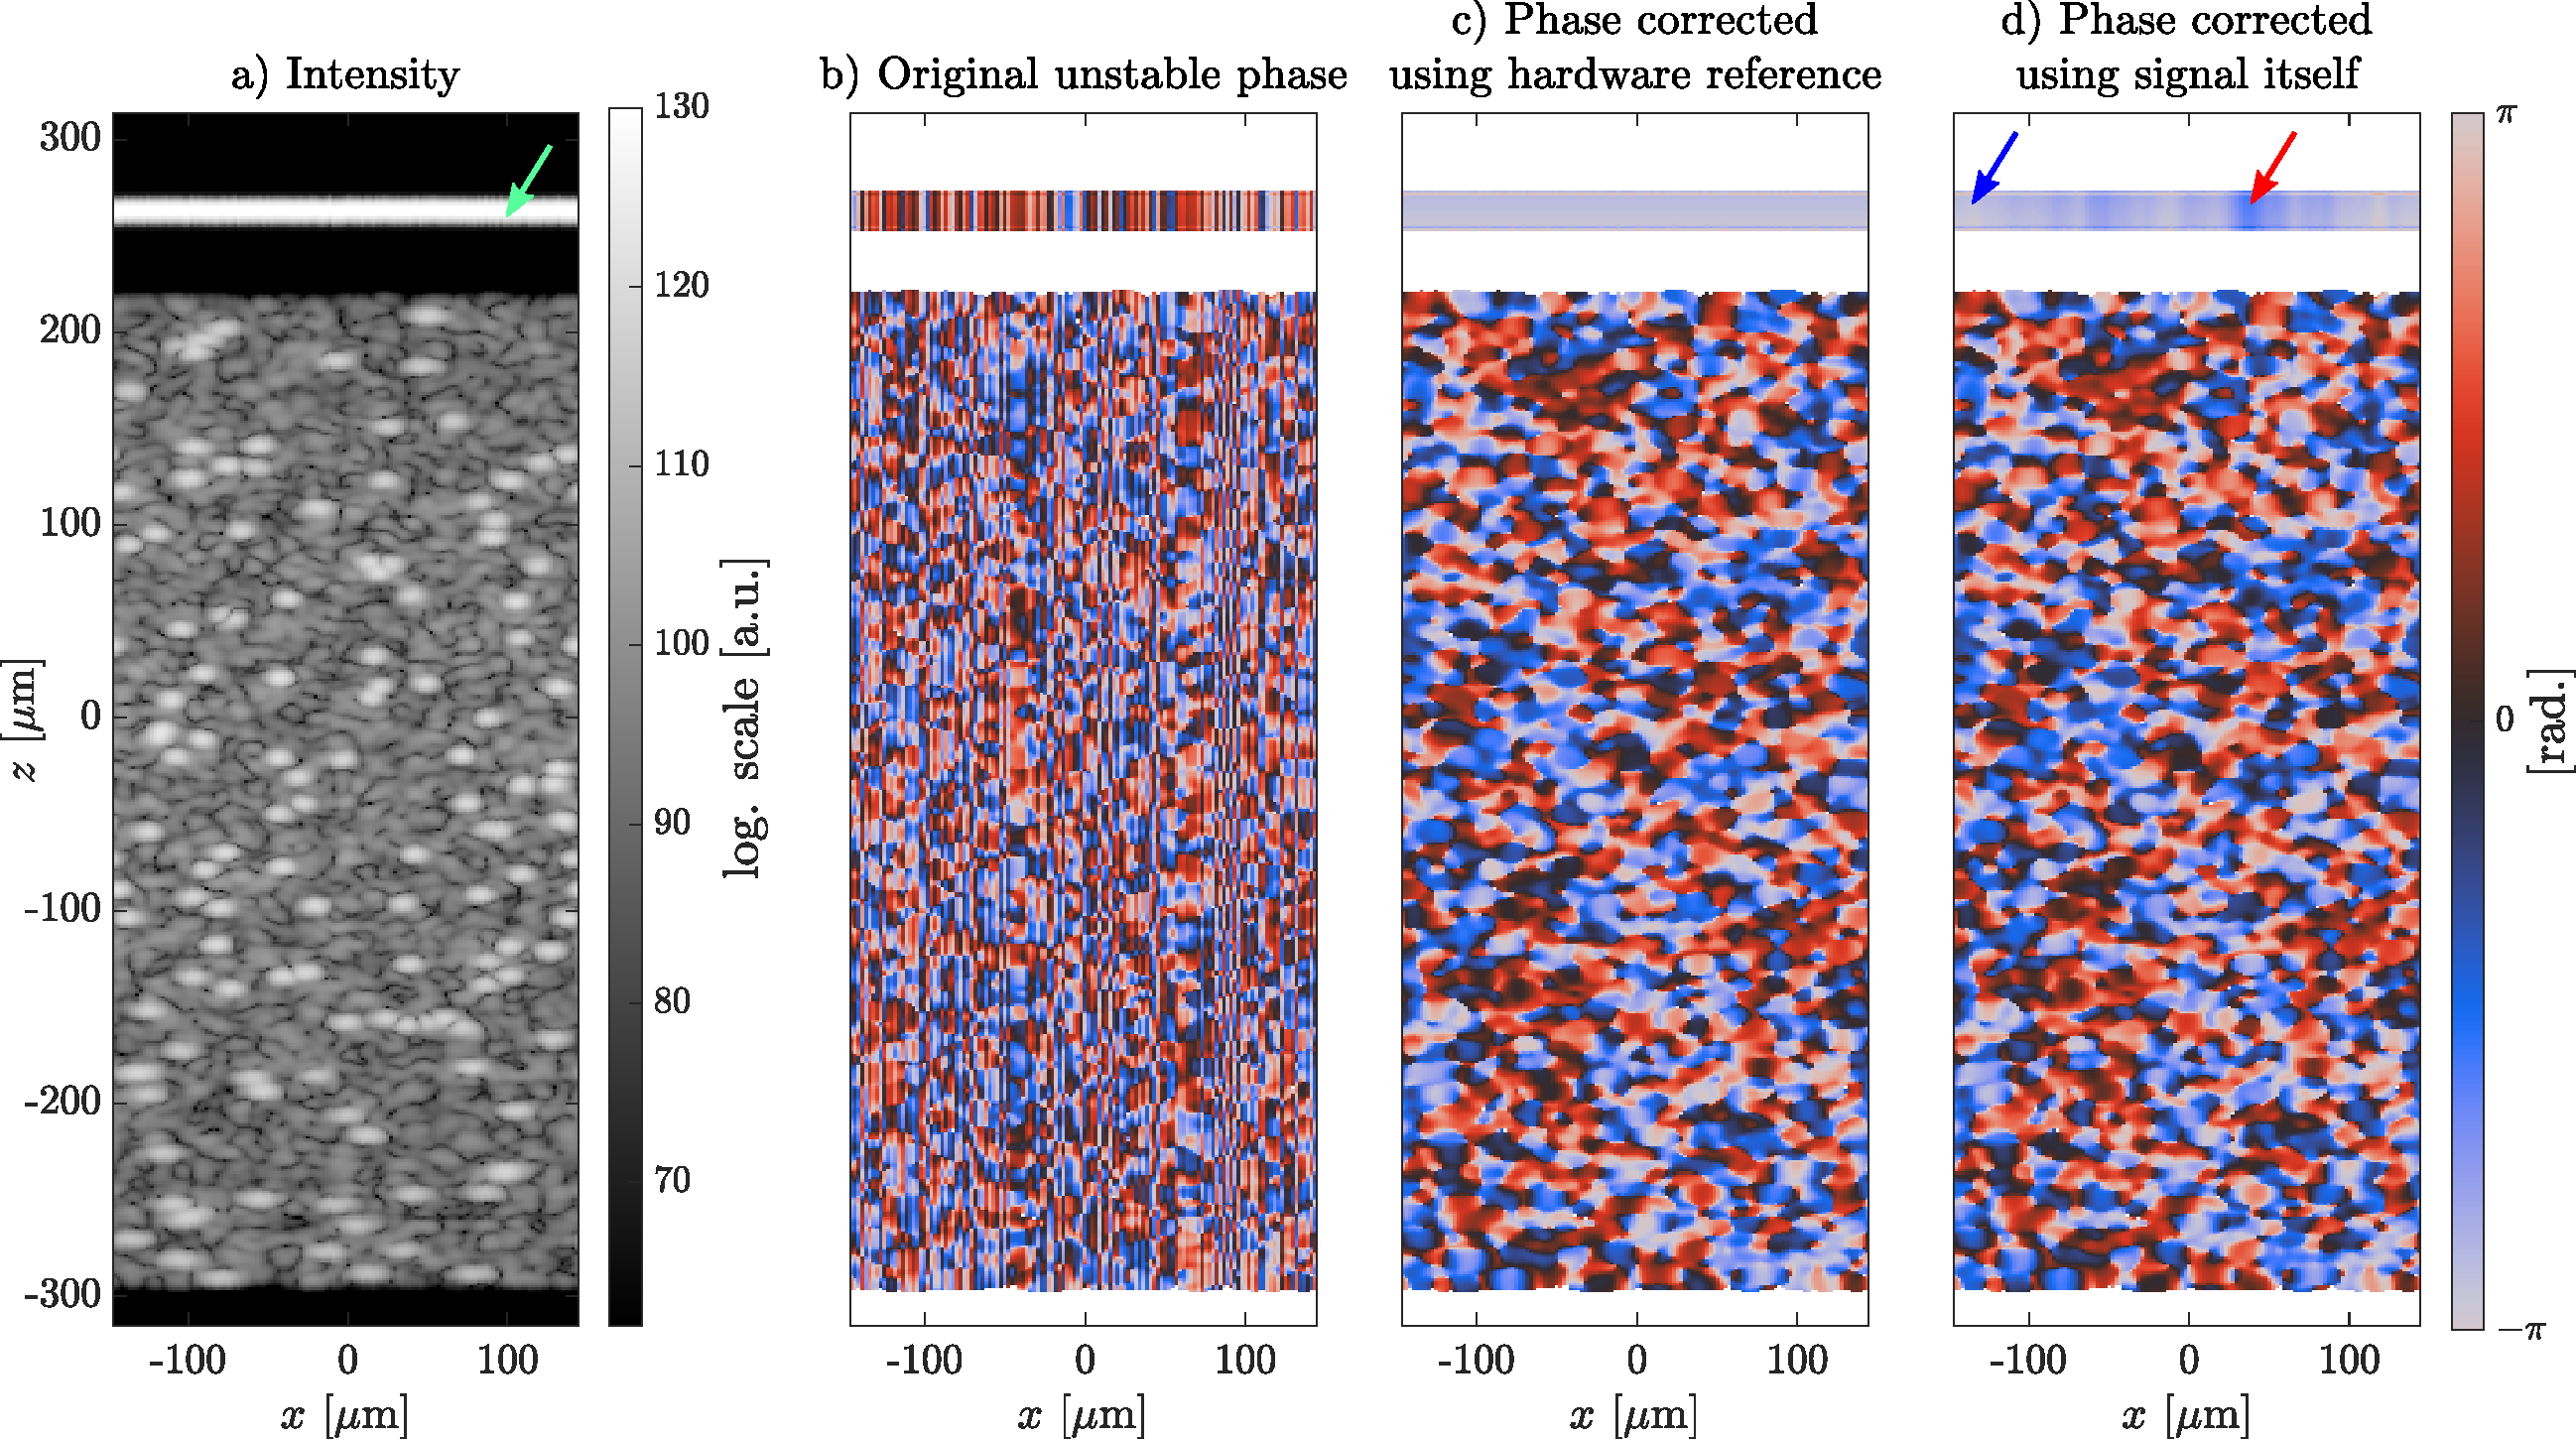
\includegraphics[width=\textwidth]{Figures/TheoreticalBasis/PhaseStabilizationComp.pdf}
	\caption[Illustration of phase stabilization.]{Illustration of phase stabilization. OCT image simulated using the forward model: (a) intensity and (b) phase presenting phase instabilities due to sample-induced phase noise. Corrected phase using (c) hardware-based stabilization and (d) fully numerical stabilization, based on tissue signal alone.}\label{fig:PhaseStabilization}
\end{figure}

Apart from the sample, a flat reflector marked by the green arrow in Fig.~\ref{fig:PhaseStabilization}(a) was added in the top of the image covering the whole fast scan axis but with a small thickness of $L=10~\mu$m. Note that phase of the reference reflector in Fig.~\ref{fig:PhaseStabilization}(b) appears constant along depth because no motion artifacts affects this direction, but it fluctuates randomly across the transverse axis due to sample-induce phase noise. This reference reflector was used to perform hardware-based phase stabilization, i.e.  computing phase differences only for pixels corresponding to the reference reflector, and the resultant corrected phase shown in Fig.~\ref{fig:PhaseStabilization}(c) exhibits a random but smooth behavior distinctive of correlated speckle, and the phase of the reference reflector is now constant as expected in a phase-stable system.

The original unstable phase was also corrected using fully numerical stabilization, employing only the signal information in the calculation of the phase differences and ignoring the pixels occupied by the reference reflector. Resultant corrected phase shown in Fig.~\ref{fig:PhaseStabilization}(d) looks fairly similar to that corrected using the reference signal, showing that indeed phase correction is possible using the sample signal alone, with no need of reference reflections. Imperfections of the method can be visualized in the phase of the reference reflector in Fig.~\ref{fig:PhaseStabilization}(d): at local scale phase is correlated as observed in the individual regions marked by arrows blue and red, but at global scale the phase is uncorrelated as noted when comparing the phase in these two regions, which in  principle should have the same value.

\FloatBarrier

In the previous models, phase differences for phase stabilization were calculated along fast scan axis $x$ but the same procedure can be applied along the slow scan axis $y$. Since its operation is intrinsically 1D, fully numerical phase stabilization yields successful results only along a single axis at a time, and its imperfections hinder any 2D correction. It means that in the presence of 2D phase instabilities in $xy$, only one axis can be phase-corrected; the one along which phase differences are calculated. Furthermore, performing two successive corrections along each axis once at a time, e.g. correcting $x$ axis first and then $y$ axis, is not successful either, as will be demonstrated later, because the global errors induced in the first correction makes impossible to correct along the second axis without destroying the phase stability in the first axis.

Apart from using a hardware reference signal which relies on physical modifications, there is not any fully numerical phase stabilization method capable of correcting phase noise in two dimensions. This limitation has been overcome using systems that provide at least phase stability along one scan axis~\cite{Ginner2017_Noniterative, Shemonski2014_Threedimensional, Fechtig2015_Highspeed, Ginner2018_Holographic, Leitgeb2016_Digital,Yasuno2006_Noniterative, South2019_Local}, in some cases even phase stability along the two scan axis is obtainable and therefore phase stabilization is unnecessary~\cite{Kumar2013_Subaperture, Hillmann2016_Aberrationfree, Pande2016_Automated, Kumar2015_Anisotropic,Sudkamp2018_Simple}. In particular, CAC techniques has been used mostly in SDOCT systems that have potential to provide 1D, or even 2D phase stability using fast line-field systems. In raster scan SDOCT systems, scanning speed along fast scan axis is fast enough to neglect motion artifacts in that direction, and phase offsets are only significant along the slow scan axis, this, in combination with numerical stabilization is sufficient for the operation of CAC techniques~\cite{Shemonski2014_Threedimensional}.

Numerical phase correction of phase-jitter noise is straightforward with extensions of the aforementioned phase stabilization methods, but they still provide 1D phase stability and no 2D phase correction is yet known. Because SSOCT are intrinsically 2D phase-unstable in the presence of phase-jitter, CAC techniques in such systems have relied on hardware solutions. For instance, full-field systems have been used since they provide intrinsic 2D phase stability given the parallel acquisition of the entire transverse plane~\cite{Kumar2013_Subaperture, Hillmann2016_Aberrationfree}, and more recently operation in raster scan systems has been possible using $k$-clocked systems and a small FoV~\cite{Kumar2017_Invivo}. These solutions are considerably unpractical since they require major hardware components that are not present in most OCT systems. For instance, $k$-clocks require an additional interferometer and a compatible digitizer that not only increase cost but also complexity of the systems.

Computational aberration correction is a powerful tool in many scenarios but it has been very restricted by the phase stability requirement; it is not possible to carry out any CAC technique in many raster scan OCT systems. There is therefore a great interest in developing a fully numerical strategies to perform CAC techniques in 2D phase-unstable system.

In following chapter, a technique for CAO in 2D phase-unstable systems developed in this work is described and successful experimental demonstrations are presented.